\documentclass[manuscript]{aastex}
\usepackage{natbib}
\usepackage{savesym}
\savesymbol{captionbox}
\savesymbol{singlespace}
\savesymbol{doublespace}
\usepackage{caption}
\usepackage{wrapfig}
\usepackage{setspace}
\usepackage{array}
\usepackage{subfig}
\usepackage[utf8]{inputenc}
\usepackage{gensymb} % general symbols
\usepackage{graphicx} % display figures
    \graphicspath{ {figures/} } % to make list of figures
\usepackage{amsmath} % equations
\usepackage{float} % figure floating
\usepackage[english]{babel}
\bibliographystyle{aasjournal}
% change margins
\usepackage[margin=1in]{geometry}
\usepackage{tabu}
\usepackage{indentfirst}
\usepackage{footmisc}
\renewcommand*{\footnotelayout}{\small}

\setcounter{tocdepth}{3}

%%%%%%%%%%%%%%%%%%%%%%%%%%%%%%%%%%%%%%%%%%%%%%%%%%%%%%%%%%%%%%%%%%%%%%%%%%%%
\slugcomment{AST Ph.D Qualifier Research Report}
\newcommand{\myemail}{vlb9398@g.rit.edu}
\shorttitle{TIME: Tomographic Ionized-Carbon Mapping Experiment}
\shortauthors{Victoria L. Butler et al.}

\begin{document}

\renewcommand{\thepage}{\roman{page}}
\title{The Epoch of Reionization and the Evolution of Large Scale Structure: Scientific Impacts of the Tomographic Ionized-Carbon Mapping Experiment}
\author{Victoria L. Butler\altaffilmark{1}}
\author{Advisor: Michael Zemcov\altaffilmark{1}}
\altaffiltext{1}{Astrophysical Sciences and Technology, College of Science, Rochester Institute of Technology, Carlson Center for Imaging Sciences, Rochester, NY}

\begin{abstract}
The study of clusters through the kinetic Sunyaev-Zeldovich Effect (kSZE) can yield insights into gas physics and cosmology that are far less susceptible to redshift effects and gas modeling than other techniques, including but not limited to feedback, cooling outflows, hydrodynamical evolutions, and the role of dark matter in cluster evolution. This effect arises from the interaction of electrons with Cosmic Microwave Background (CMB) photons due to the bulk flow of galaxy cluster gas. When studied over large volumes in both spectral and redshift space, the kSZE can effectively map the peculiar velocity field caused by the gravitational potential wells of these superstructures, and reveal the role of dark matter in large scale structure evolution. 

Previous ground based instruments that have attempted detection of this effect have done so in only a handful of individual clusters, preventing any insights into dark matter and gas physics. This is mostly attributed to foreground contamination by atmospheric emission and systematic noise. A new instrument, the Tomographic Ionized-Carbon Mapping Experiment (TIME), is designed to employ a driven-scan intensity mapping technique using a linear array of bolometers. Improvements over previous instruments are dedicated atmospheric channels to effectively reduce atmospheric noise, remove radio point source contamination, and increased mapping speed over traditional interferometric methods. TIME will complete dedicated kSZE scans of several clusters at a higher signal to noise ratio than previous instruments. In addition, TIME will make measurements of the CII and CO line emission for high redshift galaxies in order to determine both neutral and ionized gas evolutions of the ISM and IGM through the Epoch of Reionization and the Epoch of Peak Star Formation. The creation of a high redshift gas census will measure the growth of ionization bubbles around primordial galaxies, and provide insight into the properties of the first ionizing sources.
\end{abstract}

% TABLE OF CONTENTS
\newpage
\tableofcontents
\listoffigures
\listoftables

\newpage
\renewcommand{\thepage}{\arabic{page}}
\setcounter{page}{1}

\section{Introduction}

 Advances in the field of astronomy are inevitably linked to the technological advancements that are, in many cases, created specifically for astrophysical research. One such advance will happen in 2020 when JWST launches and replaces the Hubble Space Telescope as the pioneer in optical and near-IR research. Ground based telescopes have mirror sizes that are increasingly larger in diameter, with the largest currently under construction the 24.5 meter segmented primary mirror at the Giant Magellan Telescope. In comparison, the next largest segmented mirror telescope used regularly is the Keck interferometers, each with equivalent mirror sizes at 10 meters. Continuous upgrades to detector technology in concert with telescope modifications have allowed for faster data acquisition, higher signal to noise ratios, and higher resolution imaging. This combination provided deeper fields of views to fainter objects, and allowed resolution of the interiors of high redshift galaxies, to name but a few benefits. 
 
 The field of Cosmology is no exception to this trend. Instruments researching the Cosmic Microwave Background (CMB) received three distinct upgrades as they cycled through first the Cosmic Background Explorer (COBE), the Wilkinson Microwave Anisotropy Probe (WMAP), and finally Planck. COBE made the first full sky measurements of the CMB anisotropies, while WMAP and Planck increased their sensitivities to the same temperature variations but at much smaller angular scales. Finely tuned determinations of parameters such as the baryonic energy density were made possible by these upgrades, and the understanding that the majority of matter in the universe is non-baryonic. Some secondary features of the CMB were also measured to high significance, such as gravitational lensing due to large scale structure, and a phenomenon proposed in a 1969 paper by Rashid Sunyaev and Yakov Zel'dovich, now known as the SZ Effect (SZE). 
 
 The CMB is essentially a static two dimensional screen from which extremely redshifted photons propagate through the universe from the time of recombination, and occasionally interact with intervening matter. As the universe evolved and developed baryonic structures on the scale of galaxy clusters, these photons became trapped in new radiative processes. The SZE is due to these CMB photons inverse Compton Scattering (ICS) off of the energetic intra-cluster electrons, and inducing secondary thermal distortions within the anisotropy field. This effect has two flavors, one kinetic and the other thermal, where the kinetic effect is due to the physical motion of the electrons and the thermal is due to their temperature relative to the CMB [\cite{Sunyaev1970}]. WMAP made the first tentative detection of the SZE over the entire sky [\cite{Bond2003}], and was followed up with a deliberate detection effort by Planck [\cite{Planck2013}]. The kinetic effect wasn't firmly detected until 2013, and was only measured in a single cluster [\cite{Sayers2013}]. Limited detection of the kSZE did not afford much scientific insight, and the thermal effect was not researched for its insights into cluster physics, but rather as a secondary cluster counting technique, separate from the more widely used far-IR or X-ray detection methods. Needless to say, this phenomenon has significant room for further study.
 
This paper overviews the dedicated kSZE research that will be conducted by the Tomographic Ionized Carbon Mapping Experiment (TIME), and how this instrument will expand our current understanding of the evolution of large scale structure and the physics of stars and galaxies during the Epoch of Reionization (EOR). In addition to studying SZE, TIME will also observe the line emissions from CII and CO in extremely high redshift galaxies ($5 < z < 9$). Though the instrument was designed specifically for carbon line emission detection, the frequency range and type of detector was also optimal for measuring the kSZE, and is the primary scientific interest of the writer. However, both phenomenon and their implications will be discussed equally in the interest of completeness. 
 
Section 2 discusses the observational technique known as intensity mapping, which will be employed by TIME, in order to provide clarity on the subjects of data acquisition and analysis. Section 3 covers the scientific background of the SZE and what TIME's expected contributions will be, and Section 4 will do the same but for CII and CO detection. Section 5 will summarize the key points presented, and impress upon the reader the important role that TIME will play in the advancement of the field of Cosmology. 
 
%%%%%%%%%%%%%%%%%%%%%%%%%%%%%%%%%%%%%%%%%%%%%%%%%%%%%%%%%%%%%%%%%%%%%%%%%%%%%%%%%%
\section{TIME Primary Science Goal: CII/CO Line Emission and the Epoch of Reionization}
%%%%%%%%%%%%%%%%%%%%%%%%%%%%%%%%%%%%%%%%%%%%%%%%%%%%%%%%%%%%%%%%%%%%%%%%%%%%%%%%%%
\subsection{The Mysterious EOR}

The evolution of large-scale structure is something that was discussed previously in the context of mass aggregation, and understanding the role of dark matter in galaxy cluster formation. While the study of galaxy clusters is revealing, how these super structures ended up in their current state is still a debated topic. Models have been made that can simulate the clustering of matter from initial primordial fluctuations to the present day universe, but the observational evidence corroborating them have been somewhat lacking. Current evolutionary theories predict that the universe cooled to the point where elementary hydrogen and helium could form, and then cooled further to where photons decoupled from matter. This led to a period of time known as the ``dark ages'', where the universe was mostly neutral, with no emitting sources. Eventually, the initial primordial fluctuations in the hydrogen/helium gas gave rise high density regions that could collapse under their own gravity, and ignite the first stars. Because of the chemical composition and abundance of gaseous material, these ``Population III'' stars are assumed to be super massive and short lived compared to their present day counterparts [\cite{Zaroubi2012}]. This first generation of stars, and possibly some other unknown objects (micro-quasars, x-ray binaries), began reionizing the interstellar medium, and eventually conglomerated into primordial galaxies that then ionized the intergalactic medium. This is dubbed the Epoch of Reionization, where slowly, pockets of isolated galaxies developed ionization bubbles that grew with the stellar population. In addition to being ionized, the ISM and IGM also became metal rich, due to the evolution of the stars from Pop III, to Pop II and finally the present day stellar population. While this sounds like a plausible scenario, the types of objects during this time, and the growth of the ionization bubbles is still poorly understood, making the evolution of these objects to present day difficult to model accurately. If these first objects could be studied in detail for their luminosities, chemical compositions and relative number densities, the complete evolution of the universe could be mapped through the EOR, and the evolution of stars and galaxies to their current states better constrained. The problem arises in the current methods of detection. The very first luminous galaxies are assumed to be very faint, owing to their small masses and incredible distance from us, with properties similar to dwarf galaxies. Detections by both HST and ALMA are capable of probing the bright end of the luminosity function for high redshift sources, but neither are able to detect the faint dwarf population, or do so by more than a few individual detections. Individual detections of a handful of galaxies are insufficient for any global properties of the EOR to be determined. The TIME instrument will have the capability to measure the CII (doubly ionized carbon) intensity power spectrum, a tracer for the total star formation activity in high redshift galaxies, over a wide field of view and redshift space, providing the first comprehensive look at EOR galactic evolution. 

%%%%%%%%%%%%%%%%%%%%%%%%%%%%%%%%%%%%%%%%%%%%%%%%%%%%%%%%%%%%%%%%%%%%%%%%%%%%%%%%%%%%%%%%%%%%
\subsection{CII: Revelations of the EOR}
Several properties of CII make it an ideal candidate for measuring star formation for galaxies at multiple redshifts, and for constraining the EOR. For one, it happens to be one of the most abundant elements in the universe, and has an ionization energy that is smaller than that of hydrogen, at 11.26 eV. It is also one of the brightest emission lines in star forming galaxies, with a total far infrared luminosity of between 0.1-1.0 \% of the total [\cite{Stacey1991}]. By measuring the total intensity of CII of thousands of galaxies, TIME can probe even the faintest end of the CII luminosity function and constrain the EOR photon production at scales on order of  $0.01 < k < 0.3$  $[Mpc^{-1}]$  [\cite{Gong2012}, \cite{Crites2014}]. Recent measurements of individual galaxies in the far-IR, of CII emission, show a clear evolution of the gas in galaxies with redshift, indicating that something is changing about the ionizing sources of the ISM. This could be a window into the evolution of stellar populations of these galaxies, and how they are changing with time. By measuring the change of this emission with redshift, and spatial correlations, we can determine how some of the earliest populations of stars transformed their surroundings, and watch the spread of the ionization bubbles of these galaxies at various scales. 
%\begin{figure}[h!]
%\centering
%\captionsetup{width=0.8\textwidth}
%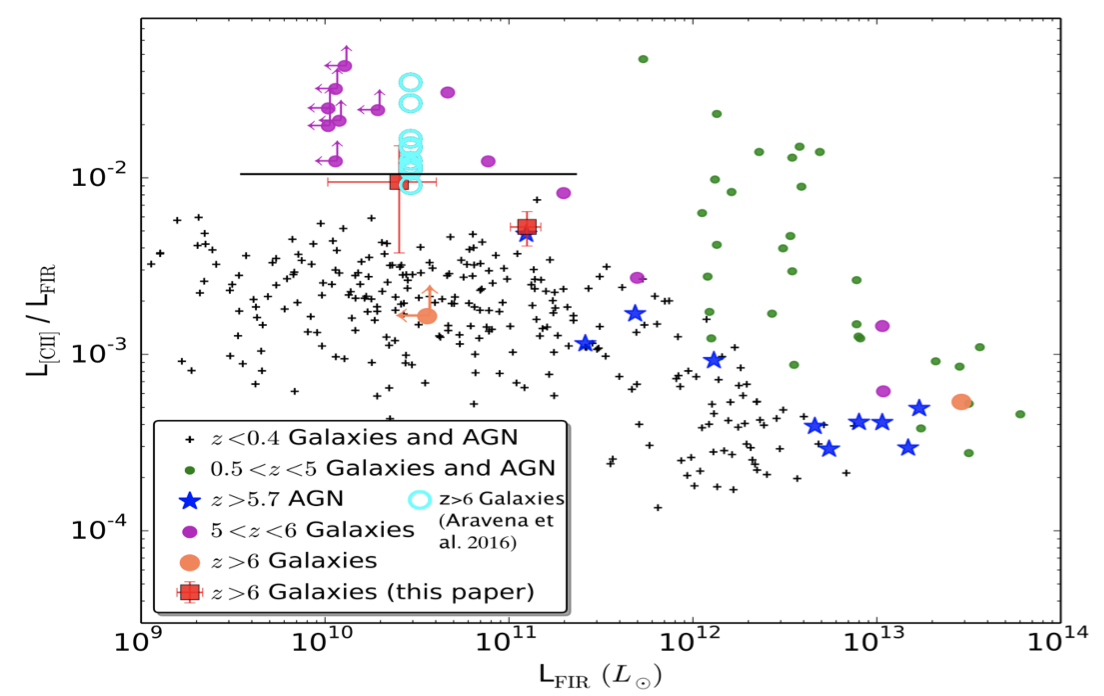
\includegraphics[width=0.8\textwidth]{gong3.png}
%\caption[CII measurements from various sources and expected emission for EOR galaxies. -(Bock et al 2011)]{A recent collection of individual galaxies whose CII emission has been measured. The black line indicates the expected CII emission for galaxies at redshifts near the EOR. [Bock et al 2011]}
%\end{figure}

In order to understand exactly what detection at different limits means for the underlying physics of high-redshift galaxies, we must also understand the physical mechanisms involved in CII production. This is even more critical for large scales, since the interaction with CII and it's ionizing environment changes depending on whether it's detected in the ISM or IGM. In the ISM, there are normal radiative processes, like spontaneous and stimulated emission that could account for the ionization, however there is also collisional excitation and de-excitation, the dominant processes depending on the number density of atoms and the gas temperature. Additionaly, the ionizing particles can be either electrons, but also neutral hydrogen, since it will have a different critical density. The CII critical density is believed to be near 100 $cm ^{-3}$ , while for hydrogen this value is closer to $10^{3} - 10^{4}$  $cm^{-3}$ .  An assumption of complete ionization of the ISM would create an electron ionizing dominant process for CII emission. [\cite{Gong2012}]. 

For the IGM, the story is slightly different, due to the varying gas physics at work. The IGM is naturally a more diffuse environment, and much less heavily ionized due to the lack of stars. This decreases the relevance of the collisional processes, and increases the important of the radiative processes, like spontaneous emission and stimulated absorption. These processes are influenced by CMB photons, which now that the ionization fraction and gas density has gone well below the critical values, are more influential to the CII ionization. An added process which can create a fine structure transition is UV pumping, although it is mostly limited to high redshift galaxies, where the first stars and quasars provide energy at wavelengths perfect for exciting the carbon atom to re-emit at the CII frequencies. Both of these mediums contribute to the observed line intensity of CII, but must be modeled carefully according to their unique environments. 

\cite{Gong2012} has generated some analytical functions to determine what the CII intensity would be for various redshifts, and also to determine the total power spectrum, as would be observed by TIME. In order to understand their result, it is useful to see how the properties that were just discussed have been included in the calculation. The following derivation is taken from \cite{Gong2012}, which starts by writing the radiative transfer equation, which reads \(\frac{dI_{\nu}(z)}{ds} = j_{\nu}(z) - \alpha_{nu}(z)I_{\nu} - 3 \frac{H(z)}{c}I_{\nu}\) . The first and second terms being radiative emission and absorption respectively, while the last term is a correction for the expansion of the universe. The first two right hand terms take the traditional forms \(j_{\nu}(z) = \frac{h\nu_{ul}}{4 \pi} n_{u}(z) A_{ul}\phi(\nu)\) and \(\alpha_{nu}(z) = \frac{h\nu_{ul}}{4 \pi} \phi(\nu)(n_{1}B_{lu} - n_{u}B_{ul})\). In this case, $\phi(\nu)$ is the line profile with redshift where \(\phi(\nu') = \phi[\nu_{0}(1+z')] = [(1+z)/\nu]\delta(z'-z)\),  and $A_{ul},B_{lu},B_{ul}$ are the Einstein coefficients for spontaneous emission, stimulated emission, and absorption. The energy for a photon is also included. This encapsulates the processes, energies, and universal properties at work. The final form of the first equation experiences a change of variables from line of sight to redshift, and then is integrated to form Equation 7. The value of the number density for the various population states is taken from deriving the statistical balance relations for the ISM and IGM. 
\begin{equation}
\Delta I_{\nu} = \frac{h c}{4 \pi H(z) (1+z)^{3}} A_{ul} f_{CII}^{grd} n_{CII}(z) \times \frac{g_{u}}{g_{1}} exp(-T_{\star,ul}/T_{S,ul})[1-\frac{exp(T_{\star,ul}/T_{S,ul}) - 1}{(2h\nu^{3}/c^{2}I_{\nu})_{\nu_{ul}}}]
\end{equation}
This can further be reduced by making an assumption that the spin temperature of the total CII intensity is much greater than that of the CMB and equivalent temperature of the level transition, then 
\begin{equation}
\Delta I_{\nu} = \frac{h c}{4 \pi H(z) (1+z)^{3}} A_{ul} f_{CII}^{grd} n_{CII}(z) \frac{g_{u}}{g_{1}} 
\end{equation}
In order to arrive at a final solution, some estimates have to be made about  $f_{CII}^{grd}$, the number of atoms in the ground state, and $n_{CII}(z)$ the number density of CII ions at various redshifts. Estimating the number of ions in their ground states is relatively easy through an estimate of the spin temperature of the gas with respect to the CMB, since in certain limits, fractional values can be found. This also happens to vary depending on whether or not the ions are in the ISM or IGM, since it is linked to the gas clumping of both mediums. These parameters can be estimated through simulations of galaxies based on observational data taken from ALMA and Herschel, but decent estimates can also be taken from nearby galaxies and solar abundance values of carbon. The estimated values for the ISM and IGM are used with Equation 8 to generate the following two plots.
\begin{figure}[!ht]%
    \centering
    \subfloat{{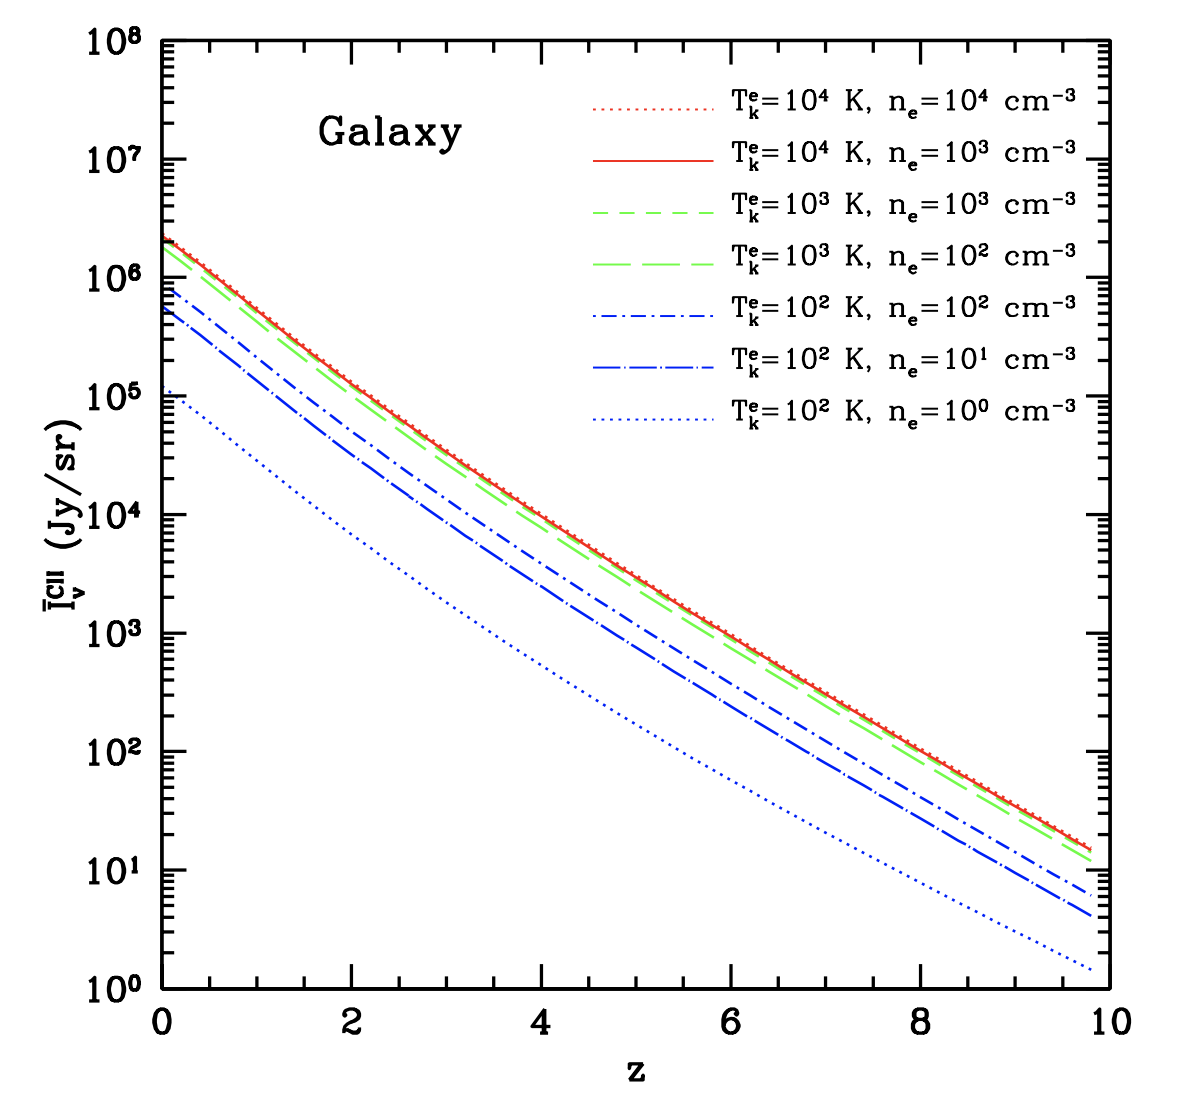
\includegraphics[width=0.4\textwidth]{gong1.png} }}%
    \qquad
    \subfloat{{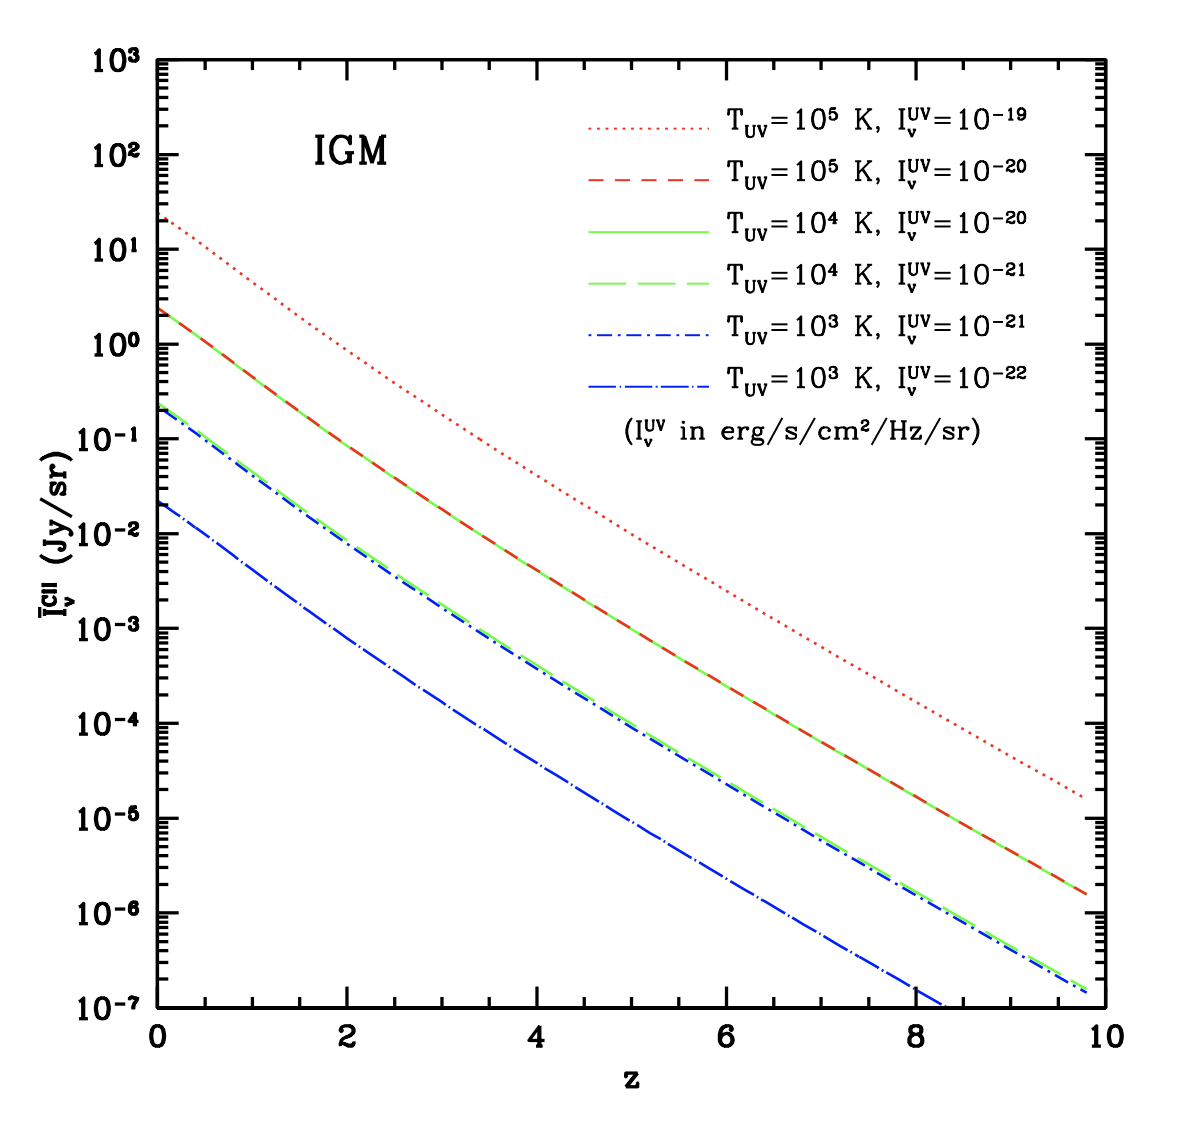
\includegraphics[width=0.4\textwidth]{gong2.png} }}%
    \singlespace
    \caption[Calculated line intensities for CII in the ISM and IGM. -(\cite{Gong2012})]{Left: The expected line intensity of CII for values consistent with the Milky Way ISM at varying redshift, electron temperature, and gas density. Right: Same as left but with IGM parameters substituted. It is clear that the CII intensity in both cases saturates at some critical value, and that the IGM does not contribute as significantly to the overall CII emission [\cite{Gong2012}].}%
    \label{fig:example}%
\end{figure}

These plots reveal that the CII intensity is predicted to have an increasing trend with redshift, and that the signal is high enough to be detected above shot noise and cosmic variance in the total CII power spectrum. The power spectrum also reveals the distribution of galaxies during re-ionization, and can reveal how matter was clumped to produce the strength of emission observed. It should be noted that the above analytical model agrees well with simulations of galaxies that tune their parameters to match those of observations. However, one physical affect that has not yet been taken into account is line contamination from foreground sources. The rotational and vibrational transitions of CO molecules at low redshift have a similar intensity to those of CII at high redshift, and can contaminate the assumed detection of CII. CO lines  can add as much as 2-30\% change in the apparent CII brightness, leading to incorrect assumptions about the physics of the ISM [\cite{Gong2012}]. Contamination by CI and NII are also present, but not to the same degree as CO. The expected detection of CO and CII by TIME is plotted below [\cite{Crites2014}].

\begin{figure}[h!]
\centering
\captionsetup{width=0.7\textwidth}
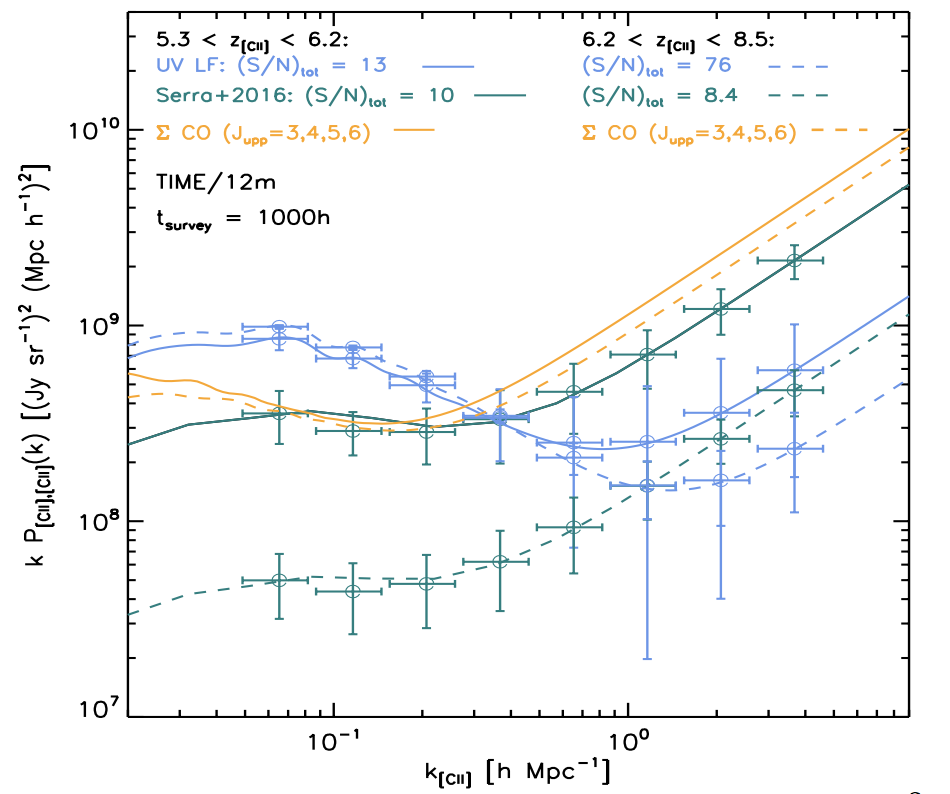
\includegraphics[width=0.7\textwidth]{bock1.png}
\caption[The expected power spectrum for CII and CO using TIME. -()]{The expected power spectrum for CII and CO using TIME. [\cite{Crites2014}]}
\end{figure}

%%%%%%%%%%%%%%%%%%%%%%%%%%%%%%%%%%%%%%%%%%%%%%%%%%%%%%%%%%%%%%%%%%%%%%%%%%%%%%%%%%
\subsection{Carbon Monoxide: A Star Formation Proxy}

While the word ``contaminant'' has been used to describe CO, it also may present a unique opportunity to probe a different property of the ISM, the molecular gas from which stars are formed. The CO transitions that TIME is sensitive to are present from $0.5 < z < 2$, the peak of star formation [\cite{Madau2014}] down to the more local universe.  With CO, it can be established whether the significant decline in star formation rates is due to the depletion of the cool gas reservoirs in galaxies, or from some other source. The majority of high redshift star formation data is from UV, optical and IR observations, which rely on having a minimum brightness consistent with only the most luminous of the galaxies, and most likely are not representative of the true galactic population. These sources of emission are also caused by hot ionized gas in the ISM, which is not sensitive to the cool gas reservoirs. As with CII, the method of intensity mapping can detect the faintest population that other detections can't reach, and can reveal the potential of those galaxies to produce future stars. By monitoring the cool gas of the ISM, the complete history of the rise and fall of the Epoch of Peak Star Formation can be traced, and the cosmic CO luminosity density can be mapped [\cite{Kovetz2017}]. This still depends on understanding the correlation between CO and H2, which has been a consistent uncertainty for many other scientific missions. Currently, the best conversions are done using H2 to CO conversions consistent with Milky Way measurements of gas densities, but these are not necessarily valid for high-redshift galaxies. The most common relationship used is that between the far-IR and CO luminosity which, in turn can also be related back to the total star formation rate density. 
\begin{equation}
\frac{L_{FIR}}{L_{sun}} = C_{FIR}(\frac{L'_{CO}}{K km s^{-1} pc^{2}})^{X_{FIR}}
\end{equation}
The constants $C_{FIR}$ and $X_{FIR}$ have been observationally determined, and the values are consistent across multiple redshifts. Higher redshift galaxies typically have a lower metallicity, allowing for easier dissociation of CO from a lack of shielding by dust, but a consistent H2 density. Knowing this conversion factor accurately can therefor still provide reasonable gas estimates of H2.  Far-IR luminosities have been measured with high accuracy, which makes this a feasible calculation [\cite{Carilli2013}].  $L_{FIR}$ can then be used with the Kennicutt relationship for star formation rates, which was derived through an estimation of the Schmidt law index [\cite{Kennicutt1998}], where $C_{SFR}$ is a conversion factor between far-IR luminosities and star formation rate that is observationally determined. 
\begin{equation}
\frac{SFR}{M_{sol}/yr} = C_{SFR}\frac{L_{FIR}}{L_{sol}}
\end{equation}

Equations 9 and 10 were taken from \cite{Breysse2016}, in their effort to determine SFRD from CO emission using intensity mapping.  They present a pessimistic uncertainty of 50\% in the conversion between CO luminosity and star formation, but also admit that if intensity mapping could be compared with other galactic features, this model uncertainty would decrease, with intensity mapping creating a significant improvement to the redshift dependence of CO.  

The predicted CO signal produced by galaxies of varying masses and redshifts is given by \cite{Visbal2010}, who include two terms  $f_{\star}$ and $\epsilon_{duty}$, which correspond to the halo star formation efficiency and 
duty cycle (the fraction of time it takes for the galaxy to emit detectable levels of radiation). 
\begin{equation}
L = 6.6\times10^{6}(\frac{R}{3.8\times10^{6}})(\frac{M}{10^{10}})(\frac{1+z}{7})^{3/2} \frac{f_{\star}}{\epsilon_{duty}} L_{sol}
\end{equation}
These two terms are once again based on observation and modeling, and carry their own intrinsic error. 

%%%%%%%%%%%%%%%%%%%%%%%%%%%%%%%%%%%%%%%%%%%%%%%%%%%%%%%%%%%%%%%%%%%%%%%%%%%%%%%%%%
\subsection{CII-CO Separation}
CO has the potential to make advancing contributions to our understanding of the gas reservoir of high redshift galaxies. 
\begin{wrapfigure}{r}{0.5\textwidth}
\vspace{-0.8cm}
  \begin{center}
    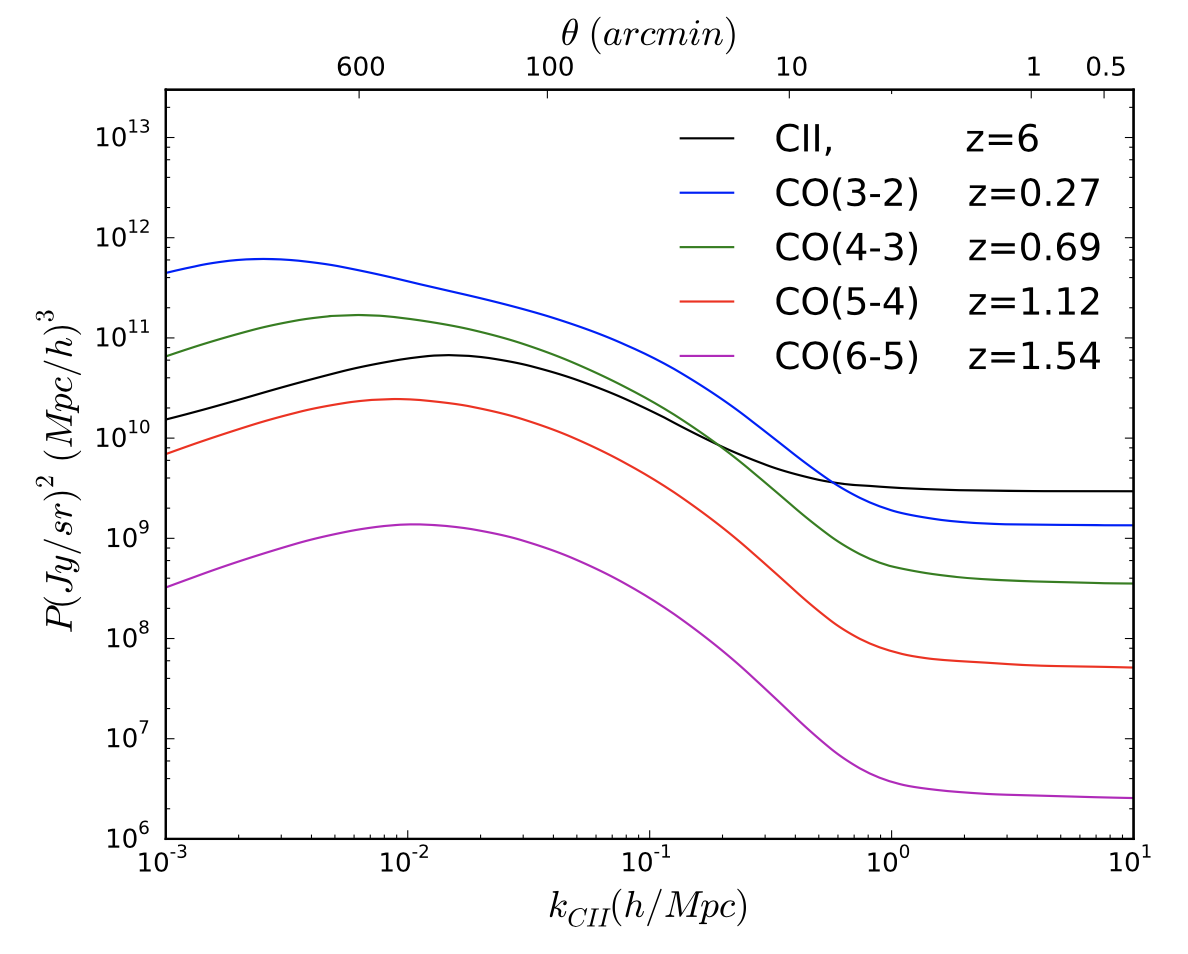
\includegraphics[width=0.48\textwidth]{cheng1.png}
  \end{center}
  \caption[Calculated CO and CII power spectrums, showing the difficulty in separating the two signals. -(\cite{Cheng2016})]{Calculated CO and CII power spectrums for a simulated universe, with the apparent mixing of the signals at various scales for specific CO transitions. [\cite{Cheng2016}]}
\end{wrapfigure}
However, since the CII and CO intensities are confused for high redshift measurements, no insights will happen unless the two signals can be disentangled (see Figure 6). Two distinct methods have been proposed by the TIME group to accomplish this task. This can in part be accomplished through correlations of the estimated CO signal with other metrics such as far-IR. As was discussed above, some empirical relationship exists between the CO and far-IR luminosity, which can be used to separate it from the CII intensity.  

A more complicated, but slightly less model dependent method is based on the geometrical separation of the two signals in power space. Both the signal for CO and CII have power spectrums that are redshift dependent, but each redshift dependence is unique. Consider a CII line intensity measured for a z = 6 galaxy with some unknown CO component, and the power spectrum is created under such an assumption, but the CO line intensity is actually from a z = 2 galaxy. When the transformation of the intensity to power spectrum is made under the z = 6 assumption, the CO dependence on redshift will be incorrectly assigned, and show a pattern which is inconsistent with the ``real'' data. This is analogous to thinking about the intensity of the lines within their own frame. To an observer at z = 6 and z = 2, the CII and CO line intensities respectively, appear isotropically emitting. However, if this CO line is transformed to a z = 6 frame, the signal becomes anisotropic and distorted, relative to the CII intensities.  

%This method relies on the apparent isotropy of the emission within its own frame, and the conversion of this emission into the comoving frame. By creating a redshift projection of the emission onto the comoving frame, the new emission has an anisotropic pattern that is dependent on redshift. However, when two emissions at two separate redshifts are transformed into the same comoving coordinates, they both exhibit different anisotropic patterns. %

An example of this technique was given in \cite{Cheng2016}, who created a realistic universe based on $\Lambda CDM$ cosmology and generated the CO and CII power spectra. Their simulated spectra is shown in Figure 6, with the mixing of the CII and CO spectrum clearly evident. The next two graphs show the change in the anisotropic patterns at z = 6. It is easy to see that the two anisotropies are projected differently onto z=6 depending on their actual redshift.

\begin{figure}[h!]
    \centering
    \subfloat{{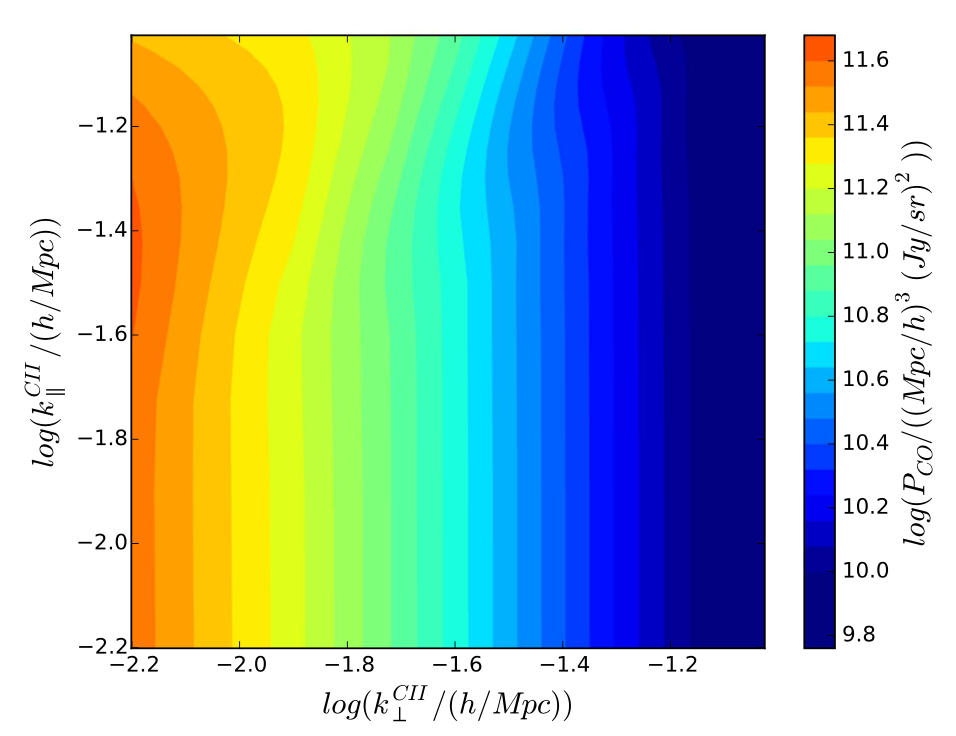
\includegraphics[width=0.45\textwidth]{cheng2.png} }}%
    \qquad
    \subfloat{{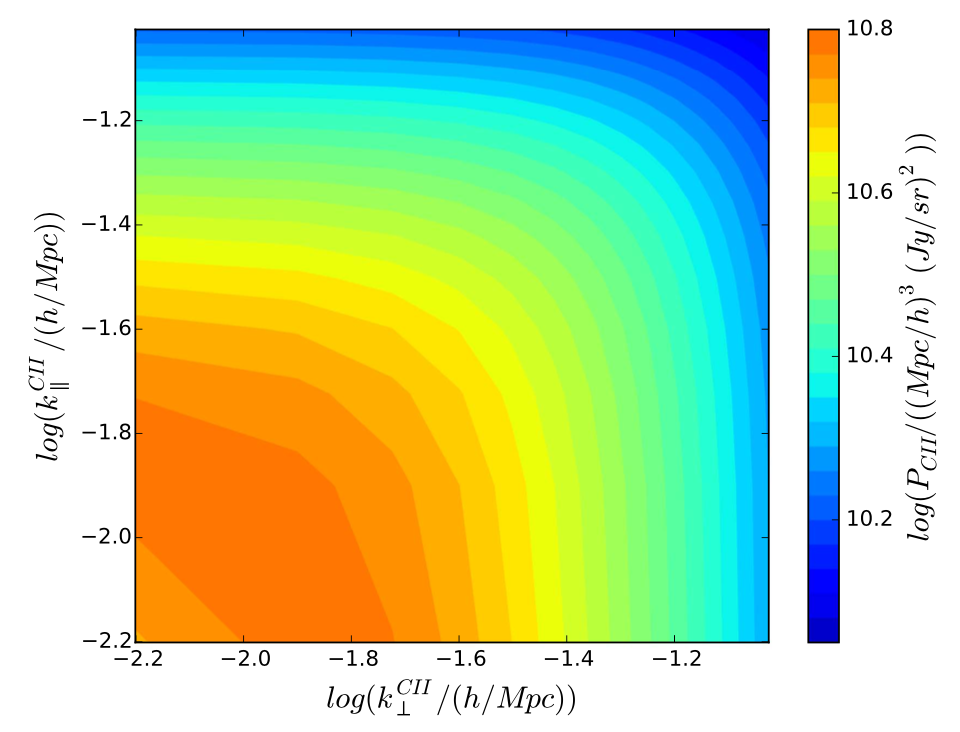
\includegraphics[width=0.45\textwidth]{cheng3.png} }}%
    \singlespace
    \caption[Deblending of the CII and CO power spectrums. -(\cite{Cheng2016})]{Deblending of the CII and CO powerspectrum. The leftmost figure is the CII power spectrum, right for CO both at z = 6. [\cite{Cheng2016}]}%
    \label{fig:example}%
\end{figure}

%%%%%%%%%%%%%%%%%%%%%%%%%%%%%%%%%%%%%%%%%%%%%%%%%%%%%%%%%%%%%%%%%%%%%%%%%%%%%%%%%%
\subsection{CII-CO-21 cm Cross Correlations}
The TIME instrument will not be conducting research into 21cm emission, however, it has been noted by some authors [\cite{Zaroubi2012},\cite{Gong2012}] that it is a useful comparator with CII and CO for determining evolutionary properties within the ISM and IGM. However, in order for it to be a useful correlator, it must also have some intrinsic scientific value, and have a relative spin temperature above that of the CMB. 21cm traces neutral hydrogen reservoirs, with a spin temperature that is highly sensitive to the physical processes at work including gas dynamics and feedback. Understanding the evolution of this tracer can lead to a more thorough understanding of these processes through the EOR. 

The 21cm line is a forbidden transition between the hydrogen triplet and singlet state, where the orientation of the spin axis is ``flipped'' between the proton and electron. While the spontaneous emission of this line has a decay on order $10^{7}$ years, the high abundance of neutral hydrogen makes this transition easily detectable. The measured intensity is sensitive to several different processes, including the absorption and stimulated emission of CMB photons, collisional excitations, and Lyman $\alpha$ pumping. These processes are incorporated into the effective spin temperature of the emitted photon, which must be of a different temperature than that of the CMB to be detected. Depending on the type of object creating the emission, this spin temperature will show fluctuations even when other parameters are held constant (such as redshift and peculiar velocity). For example, excitation from UV pumping will transfer a specific amount of energy to the surrounding atomic hydrogen depending on the energy of the photons and the optical depth of the neutral medium. Excitation due to x-ray sources however have energies too high to create 21 cm spin flips, but can cause collisional excitation due to scattering electrons. The strength of the x-ray emission will determine the energy of the collision, and how many scattering events will happen. It could also produce collision ionization and heating. By carefully mapping the intensities of 21 cm emission, the types of EOR objects ionizing the IGM can be determined [\cite{Zaroubi2012}].

\begin{figure}[ht!]
	\centering
	\subfloat{{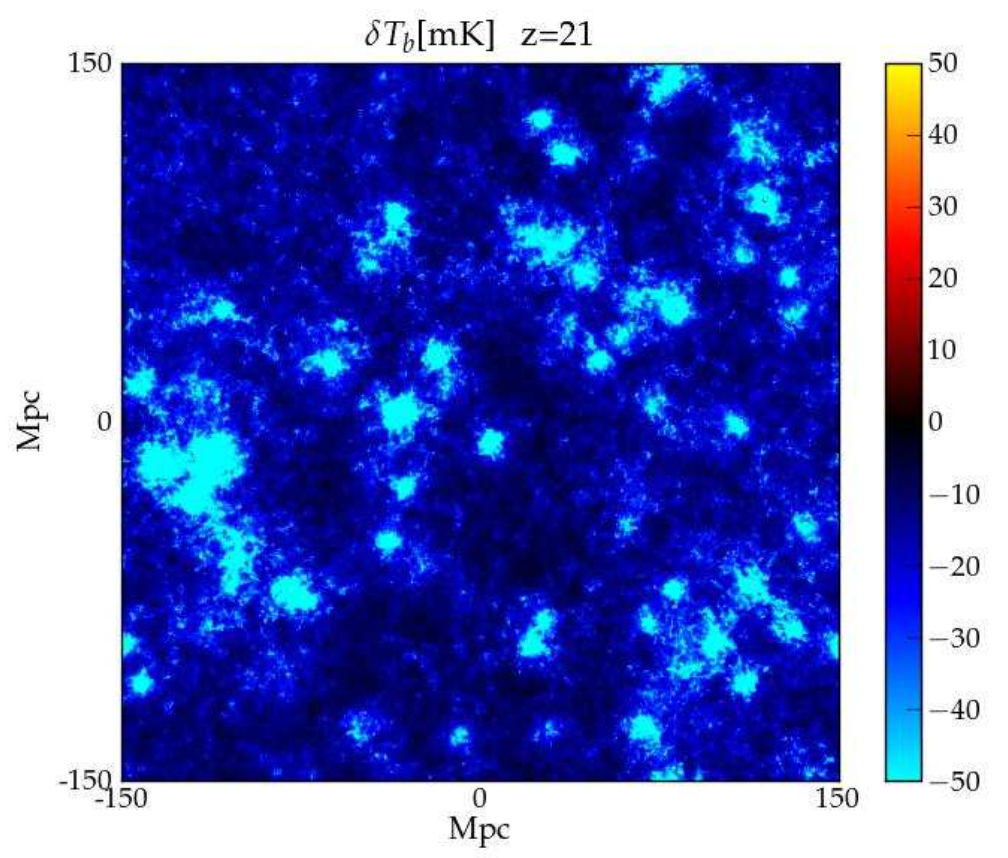
\includegraphics[width=0.4\textwidth]{santos1.png} }}%
	\qquad
	\subfloat{{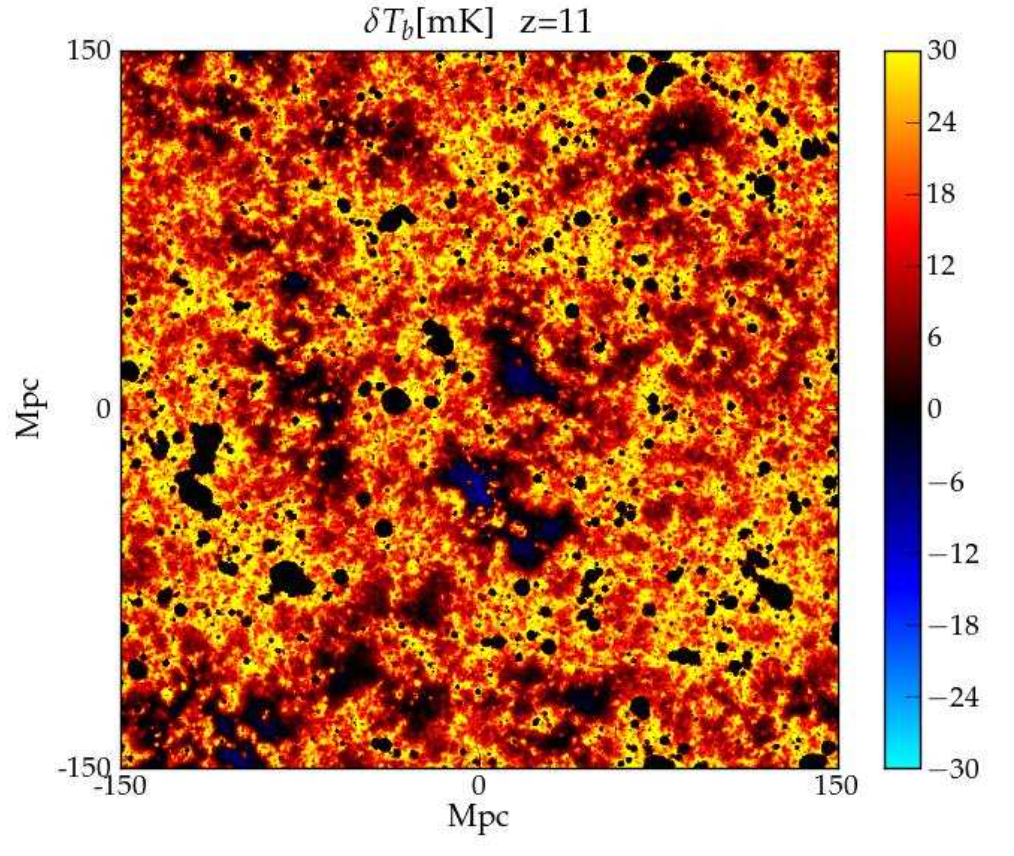
\includegraphics[width=0.4\textwidth]{santos2.png} }}%
	\singlespace
	\caption[21 cm brightness maps for different redshifts. -(\cite{Santos2010})]{Results of simulations for 21 cm brightness variations with space and redshift [\cite{Santos2010}]}%
	\label{fig: Santos et al 2010 Simulated 21cm Brightness}%
\end{figure}

As was mentioned above, a comparison between CII and 21 cm, where both are tracing the ionization history of the ISM, can be very fruitful. CII is essentially a proxy for neutral hydrogen abundances, while 21 cm probes this population directly, making it useful for corroborating CII gas mass estimates.
\begin{wrapfigure}{r}{0.5\textwidth}
\vspace{-0.8cm}
  \begin{center}
    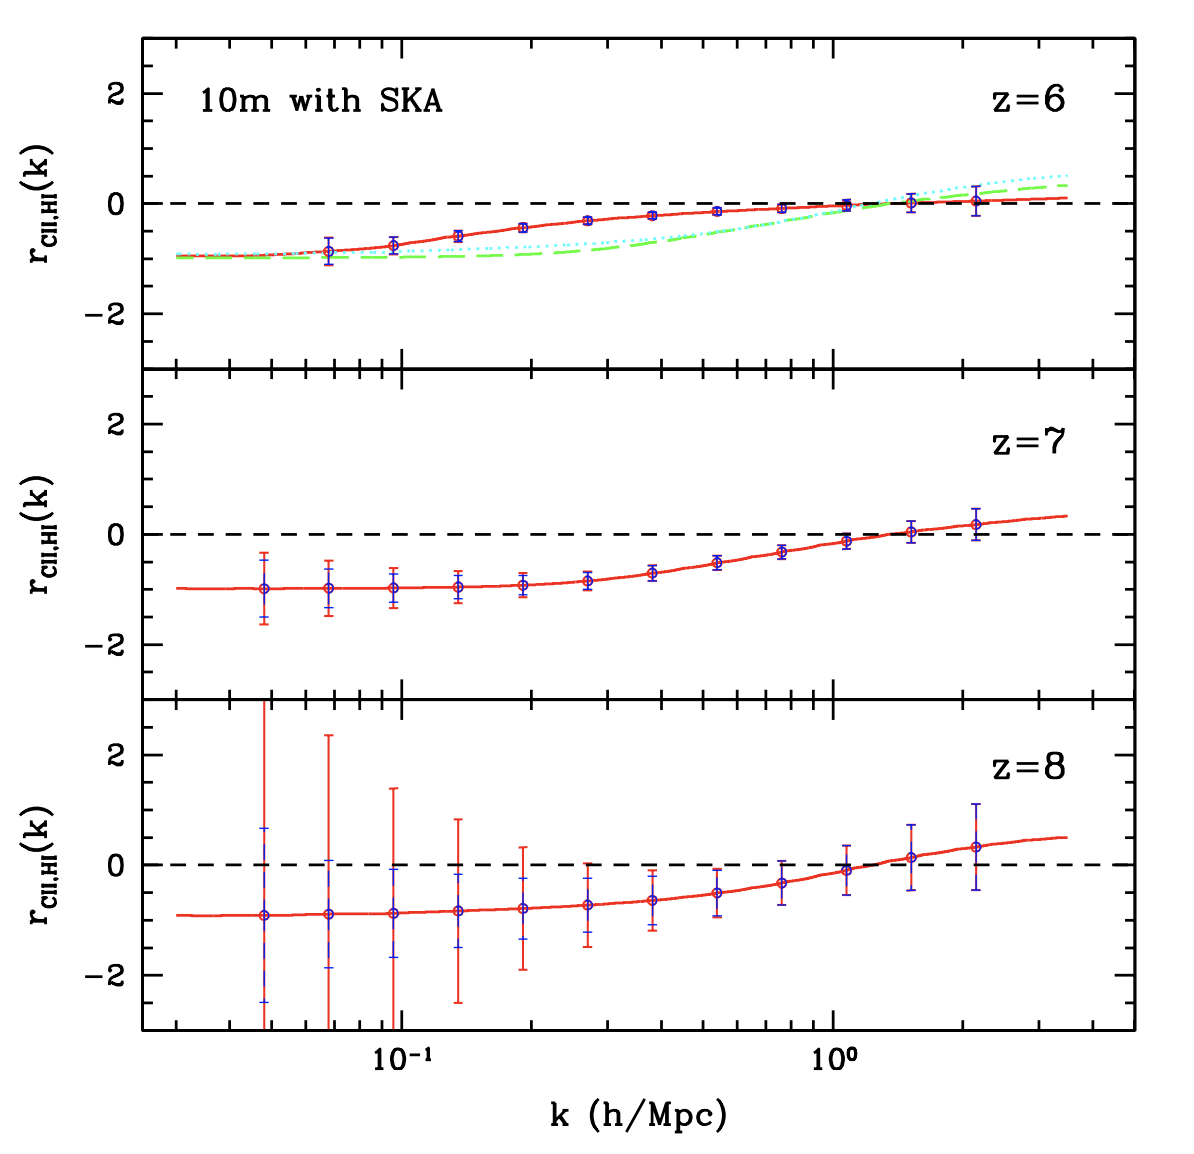
\includegraphics[width=0.48\textwidth]{gong4.png}
  \end{center}
  \caption[Cross correlation coefficient for CII and 21 cm showing ionization bubble size with redshift. -(\cite{Gong2012})]{Cross correlation coefficient for CII and 21 cm for changing scale sizes. There is a clear change in the scale of negative to positive correlation for changing redshift. [\cite{Gong2012}]}
\end{wrapfigure}
In addition, both are tracing the same density field, meaning their power spectrums will allow an angular scale determination for ionization bubble size with redshift. \cite{Santos2010} created simulated power spectra for both galaxy halo mass and 21 cm emission to predict the evolution of the EOR with redshift. The evolution of the ionization bubble size can easily be seen in Figure 8 from snapshots taken from redshifts of z = 21 and z = 11 in the simulation. It can be seen that the ionization of the ISM increases significantly, and the ionization of the IGM starts to become more complete at z = 11. 

\cite{Gong2012} coupled these 21 cm brightnesses with the expected CII intensity to create a cross-correlation coefficient calculated by \(r_{CII,HI}(k) = P_{CII,HI}(k)/\sqrt{P_{CII}(k)P_{HI}(k)}\). The mean ionization bubble size corresponds to the region where the coefficient reaches zero (from negative values) in Figure 9. For z = 6, this corresponds to a larger scale than that for either z = 7 or z = 8, consistent with the higher redshift models from the \cite{Santos2010} simulations. This particular model was created using an assumed millimeter spectroscopic survey and the 10m Square Kilometer Array. It should be noted that this same comparison can also be done with CO, but the correlation is slightly different. For large scales, CO is anti-correlated with 21 cm, since the CO implies an increase in the number density of galaxies and ionization, but a decrease in the neutral 21 cm intensity. For small scales, these two metrics are fairly uncorrelated, since CO no longer necessarily traces with galaxy counts and the neutral medium is also too small to contain a galaxy. This CO-21cm anti-correlation traces the size of large scale structure and neutral hydrogen reservoirs, allowing a determination of the ionization bubble sizes as well. 

%%%%%%%%%%%%%%%%%%%%%%%%%%%%%%%%%%%%%%%%%%%%%%%%%%%%%%%%%%%%%%%%%%%%%%%%%%%%%%%%%%
%%%%%%%%%%%%%%%%%%%%%%%%%%%%%%%%%%%%%%%%%%%%%%%%%%%%%%%%%%%%%%%%%%%%%%%%%%%%%%%%%%

\section{TIME Secondary Science Goal: The SZE and the Evolution of Large Scale Structure}

\subsection{Properties of the Sunyaev-Zeldovich Effect}

Study of kSZE has impacts for understanding both the internal gas physics and dynamics of clusters, but also for cosmology as well. In order to understand why, it is necessary to review the process by which this phenomenon is created. There are in fact two distinct flavors of the SZ phenomenon which are split into a thermal and a kinetic effect. The thermal effect is due to a thermally induced motion of intra-cluster medium (ICM) electrons, whereas the kinetic effect probes the bulk motion of cluster gas. Both, are detected as temperature fluctuations in the anisotropic signal of the CMB, and measured as a change in the intensity of the CMB signal [\cite{Sunyaev1970}].  The process by which this occurs is Inverse Compton Scattering (ICS), whereby the photons of the CMB become up-scattered by the highly energetic ICM electrons, and re-emitted at more energetic wavelengths. For the tSZE, the energy of the CMB photon is increased by a factor of \(\frac{k_{B}T_{e}}{m_{e}c^{2}}\) which in turn causes a 1mK level distortion in the CMB spectrum. This thermal effect also has the interesting property of affecting the CMB differently at different frequencies. For frequencies less than 218 GHz, the intensity of the CMB is decreased, while frequencies greater than 218 GHz the reverse is true [\cite{Carlstrom2002}]. The kSZE is due to the relative motion of the cluster gas with respect to the CMB, which creates a spectral distortion in the CMB due to the Doppler effect, induced by the cluster bulk velocity.  This distortion changes depending on whether or not the ICM electrons have relativistic energies, however, the underlying Planck Spectrum is preserved. The change in the Rayleigh Jean's temperatures is higher for positive velocities, and lower for negative velocities. For non-relativistic energies, in the rest frame of the gas, the CMB appears anisotropic, where ICS acts to create an isotropic radiation field. In the rest frame of the observer, the radiation field appears anisotropic, with the CMB photon energies increased by a factor of \(\tau_{e} v_{pec} / c\) , where \(\tau_{e}\) is the optical depth of the gas, \(v_{pec}\) is the peculiar velocity and \(c\) is the speed of light. [\cite{Birkinshaw1999}] This relationship provides a very real diagnostic tool of the internal motions of the cluster gas and significant clues about the properties of the cluster itself.

\begin{figure}[!ht]%
    \centering
    \subfloat{{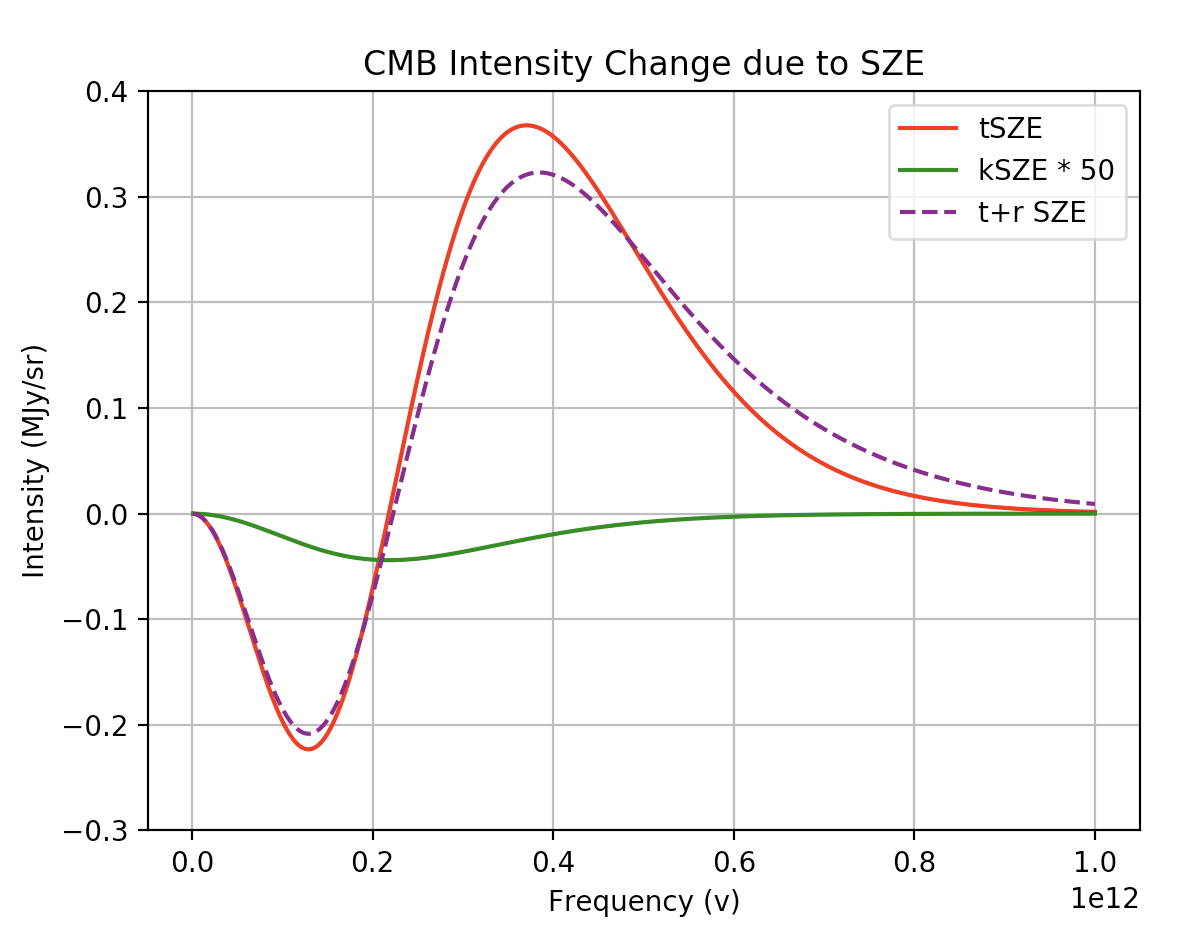
\includegraphics[width=0.45\textwidth]{tkrsze.png} }}%
    \qquad
    \subfloat{{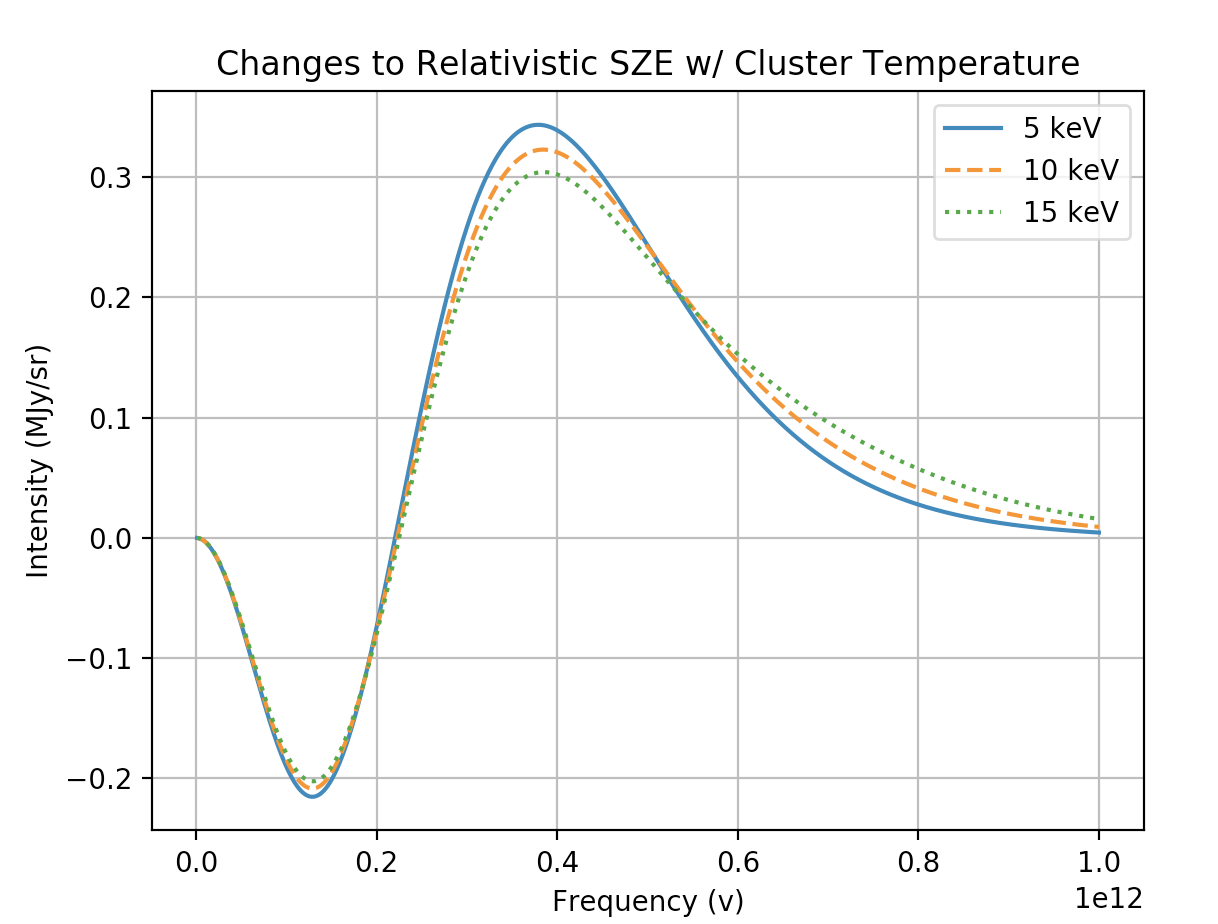
\includegraphics[width=0.45\textwidth]{rsze.png} }}%
    \singlespace
    \caption[Intensities of the kSZE, tSZE, and rSZE for simulated galaxy cluster.]{Left: Relative intensities for the SZE for thermal, kinetic, and relativistic electrons. The kSZE presents as a doppler shift in the CMB intensity and changes from positive to negative depending on the proper motion of the cluster gas. This kSZE was calculated for a clusters with peculiar velocity of -1000 km/s. The thermal effect shows a null at roughly 218 GHz but can shift depending on the properties of the cluster. The relativistic effect is for a cluster with electron temperature of 10 keV. Right: The strength of the relativistic effect at various cluster gas temperatures. The increase in the Rayleigh Jeans tail at higher temperatures makes the detection of the kSZE more attainable.}%
    \label{fig:tksze}%
\end{figure}

Although TIME science will explore primarily the kSZE signal, it is still necessary to measure the tSZE. The reason why is easily seen from Figure 1, taken from \cite{Carlstrom2002}, which shows the relative strengths of both signals in terms of the CMB brightness and the Rayleigh-Jeans brightness temperature. In both cases, the kSZE signal is orders of magnitude fainter than the tSZE, except for one special circumstance. There is in fact a null of the tSZE at 218 GHz, but for which the kSZE effect is still non-zero. This property will become fundamentally necessary for disentangling the kSZE from the tSZE. Not only is the signal much fainter, putting strict lower mass limits on the mass of the cluster observed, but the signal is further confused by CMB anisotropies that, when extracted from the full SZE signal, could remove some of the kSZE along with it. This is due to the fact that the kSZE is the first moment of the CMB, and even with careful modeling, can be difficult to remove entirely. In the case of extremely high mass, rich galaxy clusters, there is a much higher abundance of relativistic electrons, and a much better chance of retrieving a pure kSZE signal, independent of the CMB and the tSZE. For a massive cluster with \(k_{B}T_{e} = 10 keV\), modeling suggests that most electrons are well into the relativistic range. Papers of some of the earliest measured clusters found gas temperatures around \(k_{B}T_{e} = 15 keV\) [\cite{Mushotzky1997},\cite{Allen1998}], with high significance SZE detections.

\subsubsection{Redshift Independent Measurements}

Several useful applications of kSZE data were given above, however, the most powerful tool in the TIME arsenal is its redshift independent measurements. This is due primarily to the fact that the SZE for both the kinetic and thermal effect is created by photons from the same 2D surface (the CMB) scattering off of electrons in the clusters. Under the assumption that photons at the largest scales have had very little interaction with other particles until reaching a cluster, the source for the photons are all from the same redshift. To make this more abundantly clear, we can retreat back to the equation for a relativistic maxwellian distribution of electrons, like the ones that would be found in the ICM of massive clusters. Equation 3 below is taken from \cite{Birkinshaw1999} and shows the intensity change to the CMB from relativistic ICM electrons. \(P_{1}(s)\) is a scattering function for SZE,  and \(\tau_{e}\) is the optical depth for the electrons. Interestingly, nowhere contained within Equation 3 are any signs of redshift dependence.

\begin{equation}
\Delta I(\nu) = \frac{2h}{c^{2}}\tau_{e} \int_{-\infty}^{\infty} P_{1}(s) ds (\frac{\nu_{0}^{3}}{e^{h\nu_{0}/k_{B}T_{rad}}-1}  - \frac{\nu^{3}}{e^{h\nu/k_{B}T_{rad}}-1})
\end{equation}

It should be noted that while this equation is redshift independent, it does depend somewhat on cluster properties, such as assumptions that the cluster gas is optically thin, and that the temperature of the gas is in hydrodynamic equilibrium at a constant temperature. Any changes to these parameters would change the resulting spectral distortion of the CMB. The change of these cluster properties could be well modeled after the first surveys of the SZE, as it is suspected that higher redshift clusters are more compact, meaning that the gas temperature function should show a positive trend with increasing redshift. Since this equation is for a relativistic treatment of electrons, we also need a dense, hot massive cluster for it to apply, which sets a somewhat stringent mass limit for detection of the relativistic effect [\cite{Carlstrom2002}].

Fortunately, it is also possible to create an analytical function for non-relativistic electrons through the application of the Kompaneets equation [\cite{Birkinshaw1999}].

\begin{equation}
I(\nu) = \int_{-\infty}^{\infty} P_{K}(s) I_{0}(\nu_{0}) ds
\end{equation}
\begin{equation}
P_{K}(s) = \frac{1}{\sqrt[2]{4 \pi y}} exp(-\frac{(s + 3y)^{2}}{4y}
\end{equation}

\(I_{0}\) describes the blackbody spectrum of the CMB, \(P_{K}\) is the scattering function, and y is the comptonization parameter given by \(y = \int   n_{e}   \sigma_{T}   dl   \frac{k_{B}T_{e}}{m_{e}c^{2}}\) .

While this is simply theory, some of the first interferometric observations of clusters at multiple redshifts confirmed that the SZE had the same ratio to the CMB brightness across a wide range of redshifts. Figure 2, taken from \cite{Carlstrom2002}, shows this redshift-independent feature.

\newpage
\begin{figure}[h!]
\centering
\captionsetup{width=0.85\textwidth}
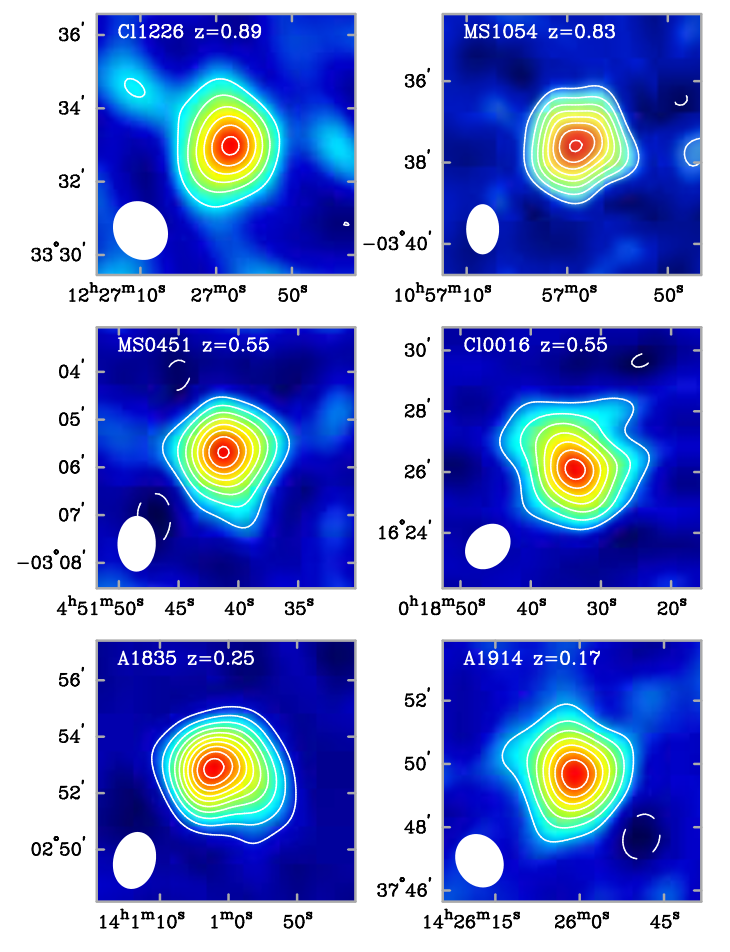
\includegraphics[width=0.85\textwidth]{carlstrom1.png}
\caption[An example of the redshift independence of SZE measurements for six different clusters. -(\cite{Carlstrom2002})]{Deconvolved interferometric SZE images for galaxy clusters between z = 0.17 and z = 0.89. Isophotal contours at multiples of \(2\sigma\) are also shown in white solid lines. In the bottom left corner, the FWHM of the beam ellipse is also shown. [\cite{Carlstrom2002}]}
\end{figure}
%%

%%%%%%%%%%%%%%%%%%%%%%%%%%%%%%%%%%%%%%%%%%%%%%%%%%%%%%%%%%%%%%%%%%%%%%%%%%%%%%%%%%
\subsection{Theorized kSZE Advances}

\subsubsection{Implications for Cosmology}

% Constraining cosmological parameters
	%(Kaiser 1987 ; Scoccimarro 2004 ; Bhattacharya & Kosowsky 2008/2009)
% Testing Homogeneity
	%(Clarkson et al 2008/2012)
% Probing dark energy properties
	%(Knox & Peel 2002)
% Constraining Lambda CDM cosmology through bulk flow upper limits
	%(Lavaux et al. 2013 ; Mak et al. 2011)
% Testing dark energy vs. modified gravity
	%(Kosowsky & Bhattacharya 2009)

It is now clear that measuring the amplitude of the kSZE in clusters is essentially measuring their bulk motions relative to the Hubble Flow. This leads to some intriguing insights into the formation of structure in the universe, and the properties of galaxy clusters in general. Research into this phenomenon also happens to occur at an opportune time, with two major unknowns plaguing the astronomical community: dark matter and dark energy. Both are vaguely understood, with their properties described in most papers by their effect on their surroundings,  and seem more well defined in mathematical contexts, such as the Friedmann Equation (FE) of state. Dark energy, or sometimes referred to as negative pressure, is one of the energy densities contained in the FE, and by current measurements appears to account for roughly 70\% of the total energy density of the universe, and might have important consequences for the late evolution of our universe. Dark matter has slightly more observational evidence, for example when looking at the flat rotation curves of galaxies, and is believed to constitute 25\% of the mass energy density of the universe.

In addition to these measurements, dark matter and energy are believed to play crucial roles in the formation of large scale structure. To understand this co-evolution, we must go back to the beginning. At the earliest point in the universes history, radiation was the dominant energy density, where subatomic particles were still coupled to the cosmic plasma. Afterwards, a brief inflationary phase magnified any quantum fluctuations in the surrounding medium and rapidly reduced the temperature to the point where atomic nuclei could form (recombination) and photons decouple. While the exact timeline has not been conclusively proven, it is theorized that dark matter production also took place at some point before decoupling, allowing baryonic matter to begin gravitational clustering, which can then be seen in the CMB anisotropies. This gravitational perturbation continued to grow and evolve as matter continued to form into first neutral atoms and molecules, and eventually to stars and galaxies. The relationship between these perturbations and dark matter is easily seen by deriving the Boltzmann Equations for cold dark matter particles. A version of a first order solution, taken from \cite{Dodelson2003}, is shown in Equation 1. Here, the overdots are derivatives with conformal time, where \(\delta\) is the dark matter overdensity, k is the magnitude of the wavevector (which in Fourier space is analogous to the three-space coordinate x), and v is the velocity of the dark matter particles. The quantities are related to the gravitational potential that the particles exert on the surrounding space-time metric.

\begin{equation}
\dot{\delta} + ikv = -3\dot{\Phi}
\end{equation}

Additionally, the overdensity of dark matter can also be related to the observed anisotropy  through Equation 2, also taken from \cite{Dodelson2003}. The variable \(\Theta_{0}\) corresponds to the monopole of the perturbation of the matter density field, at a given point from its average over all space, and the other two variables are consistent with those above. From this, it is easily seen that an overdense region produces a reduction in the observed CMB anisotropy. This is due to the the photon losing energy as it attempts to move outside of its potential well. Regions with more dark matter, and more baryonic matter, have larger potential wells, and will have a more negative anisotropy compared to underdense regions. 

\begin{equation}
(\Theta_{0} + \Phi)(k,\eta_{\star}) = -\frac{1}{6} \delta(\eta_{\star})
\end{equation}

It should be noted that this solution is valid only for large-scale modes, which is appropriate for galaxy clusters, another reason why the kSZE survey is not focused on individual galaxies. The methodology for extracting the physical properties of galaxies is much more convoluted  for non-linear regimes, as many other contaminating elements, namely dipole and quadropole fields (an example of a quadropole field being gravitational waves) create a difficult solution to the Boltzmann equations. The relationship between the anisotropies and the underlying physics of the system are much harder to correlate in that instance. 

Work has also been done to show the relationship between the emitted photons and the physics of the cluster, based on the measured CMB brightness. The equation below taken from \cite{Dodelson1995} shows the change in the CMB brightness depending on the number density of the electrons in the cluster and their bulk velocity. This first order solution to the Boltzmann Equation is derived assuming a flat, matter dominated universe, and only includes terms which are caused by the relative motion of the gas. Higher order effects have been ignored. The del's are the relative change in the CMB brightness, $n_{e}$ is the electron number density, $\sigma_{T}$ is the Thompson scattering cross section, a is the cosmic scale factor, and the $4 \mu \tilde v$ is the doppler shift term due to the motion of the electrons. The derivative is over conformal time, with the tildes denoting Fourier space. 

\begin{equation}
\dot{\tilde \Delta} + ik\mu \tilde\Delta = n_{e} \sigma_{T} a (4 \mu \tilde v - \tilde \Delta)
\end{equation}

While these equations make it apparent that studying the CMB anisotropies would lead to insights about the the dark matter densities in galaxy clusters, it also implies that anything that modifies the local gravitational potential would create deviations from the expected temperature fluctuations. The kinematic effects on the CMB photons from the bulk velocities of the electrons shown in Equation 3 show a very similar dependence to that of gravitational potentials of the clusters themselves. This leads to the conclusion that the properties of dark matter on large scales can be derived from the kSZE. Even more insights can be drawn if this effect was measured at multiple redshifts. TIME is planning on making a large scale survey of clusters and will collect data that not only contains spatial information, but also spectral. By measuring the kSZE at multiple redshifts, it will probe the history and evolution of large-scale matter density structure, and reveal how dark matter and baryonic matter interacted in the early universe.

Additional insights will be provided by the shear volume of data collected. The first attempts at measuring kSZ were done with only individual clusters. This survey can probe relationships between several different parameter spaces that others could not. For example, the process by which clusters emerge from the initial density field, and how the initial density affects the resultant mass of the cluster, which is still widely unknown. Another use is to determine whether cluster properties vary with redshift, or perhaps with other parameters such as merger rates and non-linear affects. One parameter space that is still being researched is the relationship between cluster mass and its resulting temperature. 

X-ray data has largely contributed to the knowledge of clusters, since the emission from the ICM is a much larger signal than that of kSZE. However, the conclusions that are derived from this data are significantly dependent on modeling based on the local universe. The assumptions of gas mass fraction, stellar census with age, and radiative transfer that are simulated for these clusters may not actually hold across every redshift, and cannot be confirmed without a secondary source of data. In order to make assumptions about the ratio of baryonic mass in the cluster to the total mass also relies on modeling of the clumpiness of the gas, and the assumption of hydrostatic equillibrium, both of which can also vary widely per cluster, and are a significant source of uncertainty in many measurements. kSZE provides a measurement that is independant of this type of modeling [\cite{Carlstrom2002}].

While the kSZE is a breakthrough for the study of clusters, it can also provide further confirmations of existing theory. For example, kSZE is a very good check on the current \(\Lambda Cold Dark Matter\) (\(\Lambda CDM\)) paradigm. Since it is essentially probing the growth rate of matter, it is sensitive to the the largest overdensities in the field, and therefor should fit well the model of primordial fluctuations that seek to recreate this density pattern in the CMB, under the assumed cosmology. If the number of peaks in the density field matches the well established cosmological model, it will provide an independent confirmation of the parameter space that we live in. It also provides further constraints on the modeling of the gas within the cluster. Since our measurements are extremely sensitive to the motions and temperature of the gas, (and with high enough resolution instruments, the gas mass with radius), we can determine the hydrodynamical evolution of the cluster gas with redshift, in addition to cluster mass. This could include information about evolutionary effects such as feedback and cooling outflows, and how they affect the cluster environment, specifically in the ICM. kSZE also probes the transverse component of the velocity field. When combined with imaging done through weak gravitational lensing, which is sensitive to the other two velocity components, it can create a 3D velocity map of each galaxy cluster which will allow more accurate modeling of the true shape of the cluster potential well and the cosmic filament that large structures are believed to reside in [\cite{Birkinshaw1999}].

\subsubsection{Implications for Cluster Physics}
% Include a discussion from Reiprich 2013 about why we should study clusters to begin with.

% Reconstructing gravitational potentials
	%(Knox & Peel 2002)
% Merging Clusters
	%(Diego et al 2003 ; Kock & Jetzer 2004)
% Scaling Relations to determine cluster mass
	The average mass and total number of clusters in the Universe is highly sensitive to the effects of dark energy in the distant universe, and the effects of dark matter in the nearby universe. The final number and mass is also closely tied to the primordial matter power spectrum 
	%(Benson et al. 2013 ; Rozo et al. 2010)
% Physics of the ICM
	%(TBD)

%%%%%%%%%%%%%%%%%%%%%%%%%%%%%%%%%%%%%%%%%%%%%%%%%%%%%%%%%%%%%%%%%%%%%%%%%%%%%%%%%%

\subsection{Comparison of SZE Against Alternative Methods}

% bulk flow measurements are too high or too low for existing cosmology, and many measurements don't agree
% (too low ; Itoh et al. 2010)
% (too high ; Kashlinsky 2010 ; Abate and Feldman 2012)

\subsubsection{X-Ray ICM Measurements}

(Benson 2004)
%One of the systematic effects that we are primarily concerned about in using X-ray models to fit SZ observations is that the X-ray Beta models might over-fit to the cooling core for cooling flow clusters. This is a result of X-ray observations being more sensitive to over-densities in the core of a cluster than SZ observations, because LX ? n2e while ISZ ? ne.

% Pitfalls of studying the ICM with Xrays (McNamara et al 2005; Markevitch & Vikhlinin 2007)

%for example the (1 + z)4 dimming of the X-ray surface brightness (eq. 19). In practice, however, this redshift independence is currently not fully exploitable due to finite beam sizes. Another major advantage is the linear dependence of the SZ signal on electron density, as opposed to the n2e dependence of X-ray brightness, which potentially makes it more suitable to study the low density outskirt environments.'' (Reiprich 2013) (Also reference equation 19 to show the effect of cosmological diming on the X-ray surface brightness)%

%Mrockzkowski 2012 discusses the dimming of the x-ray signal due to increase in distance. Something SZE doesn't suffer from.%

%%%%%%%%%%%%%%%%%%%%%%%%%%%%%%%%%%%%%%%%%%%%%%%%%%%%%%%%%%%%%%%%%%%%%%%%%%%%%%%%%%%%%%%%%%%%
\subsection{Previous Cluster SZE Detections \& Advancements}

The study of SZE is not a new branch in the field of Cosmology. Some of the first SZE measurements of clusters were made back in the 1970's on the Chilbolton Observatory 25 meter telescope in England, and at the Owens Valley Radio Observatory (OVRO) in California in the 1980's (\cite{Birkinshaw1999}). These instruments provided proof that SZE was detectable in massive clusters, but the results were often confusing, as measurements of the same object between different telescopes returned different cluster gas temperatures. These differing values were often not within error of each other, revealing a serious systemic uncertainty not accounted for in the analysis. At the time, so few clusters were being targeted for SZE research that it was impossible to make any global statements about the properties of the intra cluster medium, or to determine the cause of the uncertainty in the measurements. 

SZE research improved with the advent of more tailored instrumentation, and an increase in the number of clusters studied. Research into the thermal effect is now extremely common in cosmology, because of its relatively high signal compared to kSZ [\cite{Benson2013},\cite{Saliwanchik2015}],\cite{Bleem2015},\cite{Planck2016}]. Most are surveys of a large number of clusters, using basic beta modeling of the gas, with the intent to make statistical arguments for bulk cluster properties. However, these measurements utilize brute force methods that don't reveal any properties of cluster substructure (i.e. cooling flows, agn activity, mergers), leaving behind valuable information. This kind of study is interested in using SZE as a counting technique, to confirm global cosmological parameters, and reach a lower mass threshold limit for clusters at high redshift. 

Despite the ubiquity of tSZE meaurements, dedicated large scale kSZE surveys are still not realized. However, many experiments have paved the way for the TIME instrument, which will be an additional stepping block to this goal. An early example is SuZIE II, one of the first experiments to claim a 95\% confidence limit constraint on bulk flows at intermediate redshift of < 1410 km/s, in the direction of the CMB dipole. SuZIE II was a bolometer with 3 photometer bands between 150-350 GHz, which included electronic differencing of similar row and frequency bolometers, for removal of common mode atmospheric emission. The atmosphere was further removed by creating models of the observed cluster and subtracting any additional signal. Traditionally, bulk flows would be determined using peculiar velocities obtained optically, given a fairly close cluster and high resolution telescope. The distance would be estimated with photometric, or if it was available, spectroscopic redshifts, which are more subject to errors with an increase in distance [CITE REFERENCE HERE]. As explained above, SZE measurements do not suffer from redshift effects. 

The results from observing 6 clusters showed an average peculiar velocity of 150 (+430 -390) km/s , which is not a statistically significant result [\cite{Benson2003}]. In subsequent analysis, it was discovered that the results were heavily affected by differential atmospheric emission, which was not subtracted effectively by either of the above methods, leading to a modified 68\% certainty in the results [\cite{Mauskopf2000},\cite{Carlstrom2002}]. The atmospheric templates were also dependent on the modeling of the cluster gas, and were sensitive to the distribution and temperature. SuZIE II also had large beam sizes which meant low resolution, and the inability to mask point source contamination without sacrificing large fractions of data. 

In a following data release, the total clusters observed by SuZIE II increased to 15, with additional analysis of the SZ flux and central Comptonization parameter. This led to two important insights; that combining x-ray data with SZE signals could improve the results, and variations of the standard Beta model used in determining cluster temperatures radically changed the results. Central Comptonization is similar to the Compton Y parameter introduced above, but is applied at the center of the cluster, and depends on the electron density and temperature. The cluster centroid was determined using X-ray data from ROSAT, which included published models of gas density and electron temperature. However, as described previously, those values are sensitive to other processes within the cluster, such as cooling flows. When two different models were fit against the data for cluster A1689, the calculated central comptonization changed by 40\% [\cite{Holzapfel et al. 1997b}, \cite{Reese et al. 2002}]. This was because the cluster was poorly resolved by SuZIE II, and relied entirely on the assumed ICM gas model [\cite{Benson2004}]. 

Other instruments followed SuZIE II to make kSZE improved measurements of individual clusters, including Z-Spec. Rather than relying on photometry, Z-Spec utilized an R ~ 300 grating spectrometer between 185 - 305 GHz to make measurements of a single cluster RX J1347.5-1145. One interesting result from the retrieved kSZE spectrum were possible contaminants. In this cluster, there was reported a shock region to the southeast of the cluster center, along with several other subshocks. This combined with variations in the cluster shape led to difficulty in constraining an optimal isothermal beta model, since shocks and non-uniform structure change the clumping and temperature of the cluster gas. The team reported that if the beta model was changed to those used in other literature, the Compton Y value would change as much as 25 \%. The traditional beta model is given by 
\begin{equation}
    n_{e}(r) = n_{e0}(1 + \frac{r}{r_{c}}^{2})^{-3\beta/2}
\end{equation}
as is a measure of the radial electron number density of the cluster. This changes the projected radial dependence of the parameter as follows
\begin{equation}
    y(b) = y_{0}(1 + \frac{b}{r_{c}}^{2})^{1/2 - 3\beta/2}
\end{equation}
This issue of beta model dependancy is a standing problem for SZE research, and will have to be addressed again for TIME.

Z-Spec also highlighted additional uncertainties in the data, one component from the Cosmic Infrared Background, and another from varying models of the AGN present in the cluster. A simulation was run with several sub-mm sources fed through the Z-Spec data pipeline for a random patch of sky, with changes in the continuum background flux reported next to the kSZE. The result has a mean near zero, but a bias as large as 300 $\nu Jy$ if a source were in the beam. Most analysis performed for kSZE assumes that the sub-mm background is well understood. However that assumption may not hold if the cluster is significantly lensed, and could cause problems for large scale kSZE surveys of the future [\cite{Zemcov2012}].


To improve upon the discovery that the beam size of the instrument changed the dependence of the data on the cluster model, investigations by \cite{Saliwanchick2015} et al. discovered the optimal beam size for least dependence to be one the same size as the cluster. This result was obtained by first creating a simulated universe based on current cosmology, and populating it with realistic CMB background fluctuations, sub-mm clusters, radio point sources, and others. Any of the clusters created were given a standard isothermal beta profile, and were then ``measured'' in the same way as the South Pole Telescope (SPT) performed observations. The beam size across the cluster was allowed to vary, and the recovered profiles of the cluster, namely the calculated Compton Y parameter was compared to the one inputted by the simulation. The calculation is similar to the one employed by the SPT, where the source function of the SZE signal is integrated over some finite area

\begin{equation}
Y_{SZ} = 2\pi \int_{0}^{\Theta_{int}} S(\theta) \theta d\theta
\end{equation}

where $\Theta_{int}$ represents the angular aperture of the beam. Since the source template for the cluster was a perfect 2 dimensional projected $\beta = 1$ model, given by $\Delta T = \Delta T_{0}(1 + \theta^{2}/\theta_{c}^{2})^{-1}$, this integral has a simple analytical solution with familiar quantities. 

\begin{equation}
Y_{SZ}^{\theta} = \frac{\pi \Delta T_{0} \theta_{c}^{2}}{f_{x} T_{CMB}} Log[1 + (\frac{\theta}{\theta_{c}})^{2}]
\end{equation}

$f_{x}$ is the 
\begin{wrapfigure}{r}{0.55\textwidth}
\vspace{-0.8cm}
  \begin{center}
    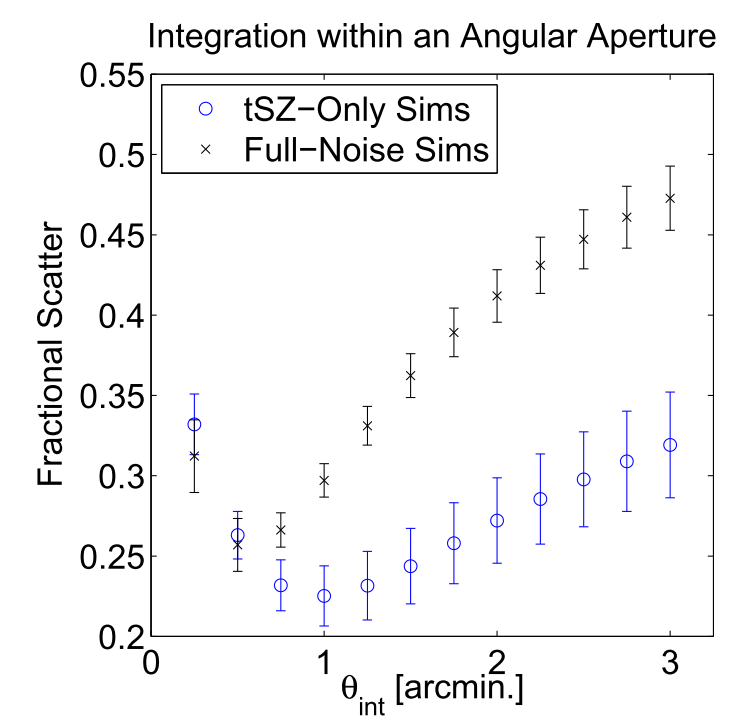
\includegraphics[width=0.5\textwidth]{saliwanchick1.png}
   \end{center}
\caption[MCMC Cluster Simulation Showing Scatter Versus Integration Angle -[\cite{Saliwanchick2013}]]{The tSZE only simulation contains intrinsic scatter of the dataset. The full scatter set includes the CMB, point sources, atmospheric, and instrumental noise. This was a simulation for clusters at a median redshift of $z ~ 0.6$[\cite{Saliwanchick2013}]}
\label{fig:sali1}
\end{wrapfigure}
relativistically corrected SZ spectrum, $T_{CMB}$ is the temperature of the CMB background at 2.73 K, while $\delta T_{0}$ is the central temperature decrement compared to the CMB. They then compared the observation data and real data to known scaling relationships and compared the scatter for both tSZE only and tSZE + Noise measurements. The results shown in Figure ~\ref{fig:sali1} clearly indicate that the least scatter from the retrieved data set is for beam sizes equivalent to the angular diameter of the cluster at the given redshift. 

%(Hand 2012):
% wasn't the first group to use multiple measurement methods, like Mrockzkowski above.
% used physical locations and velocities from SDSS compared with kSZE to determine mean pairwise momentum and were one of the first groups to conclusively determine cluster motions using the kSZE.
% showed that the cluster motion was consistent with standard cosmology, but did not determine bulk flow
% "The evidence for a nonzero mean pairwise momentum from a kSZ signal presented here can also be interpreted as a measure of baryons on cluster length scales; a deficit of observed baryons has long been a cosmological puzzle [44]. Our signal is roughly consistent with the standard baryon fraction based on primordial nucleosynthesis, given independent halo mass estimates based on clustering of our luminous galaxy sample."
% The signal in Fig. 1 represents the first measurement of the cosmic velocity field made directly with respect to the rest frame of the Universe. It is consistent with simulations based on the standard cosmological model. This signal is also the first clear evidence for the kinematic Sunyaev-Zel’dovich effect."
% We infer that our galaxy luminosity cut corresponds to a cluster halo mass limit of roughly M200 = 4.1 × 10^13 Solar Masses and a mean cluster halo mass of M200 = 6.5 × 10^13 Solar Masses."
% they made several realizations of the simulated kSZE sky map under different halo mass limits until an optimal fit to the data was found
% can only use kSZE to find line-of-sight component of the momentum, but is differential, meaning that any systematic errors associated with individual clusters gets washed out in looking for the null signal. 

\begin{wrapfigure}{r}{0.55\textwidth}
\vspace{-0.8cm}
  \begin{center}
    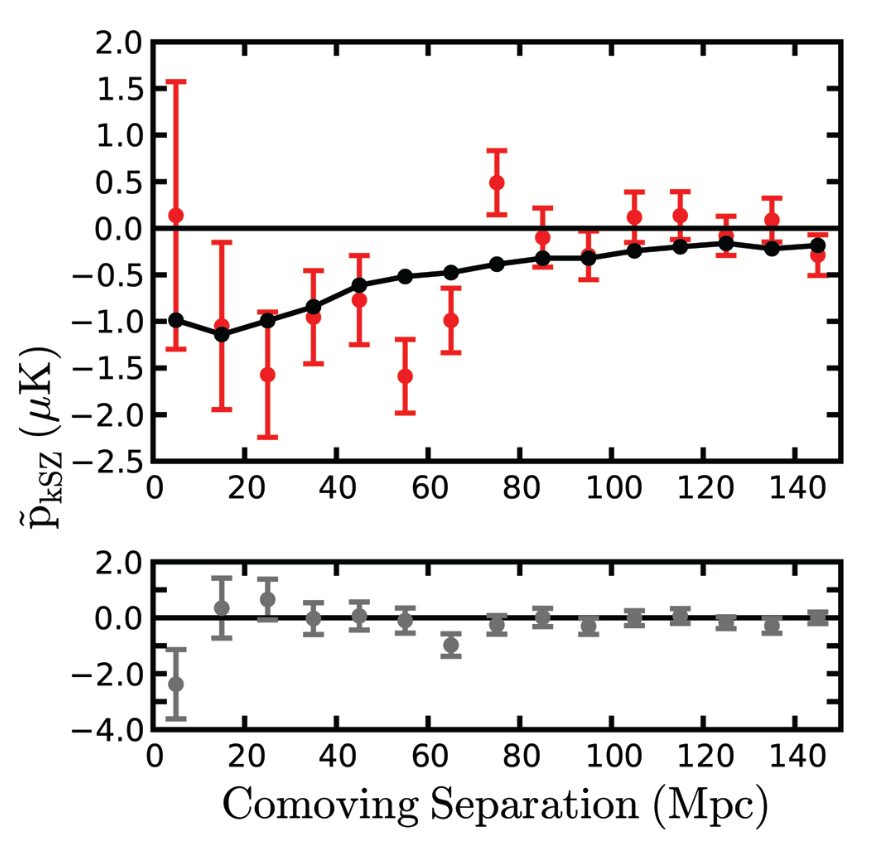
\includegraphics[width=0.5\textwidth]{hand1.png}
   \end{center}
\caption[Mean Pairwise Momentum of BOSS DR9 Selected Clusters using kSZE -[\cite{hand2012}]]{TOP: Mean pairwise kSZE signal for the 5000 most luminous BOSS DR9 galaxies in the ACT sky region, as well as a simulation for comparison. The real data set is shown in red, while the simulation, based off of large-volume cosmological simulations, is shown in black. The red data points were corrected for any redshift dependent temperature contributions, and minimizes the total Poisson and pixel noise. Errors were estimated using bootstrap resampling. BOTTOM: The probability of data given a null signal, consistent with a null signal. [\cite{hand2012}]}
\end{wrapfigure}

%(Sayers 2013): 
% along with Hand, also showed that pressure profiles were consistent with NFW dark matter halo profiles. 

%%%%%%%%%%%%%%%%%%%%%%%%%%%%%%%%%%%%%%%%%%%%%%%%%%%%%%%%%%%%%%%%%%%%%%%%%%%%%%%%%%
\subsection{Expected TIME SZ Measurements}

% include discussion on atmosphere from Sayers paper here
(Sayers 2013):
%"As detailed in Section 4.1, a model is required to interpret our SZ data because the large-angular scale atmospheric noise necessitates high-pass filtering of the data, which removes signal on large angular scales. As a result, a spatial model of the SZ is the only way to recover this large-scale signal in order to obtain an absolute surface brightness."
%To remove atmospheric fluctuations from the data, we first subtract a template of the common mode signal over the FOV, and we then high-pass filter (HPF) the time- stream data at 250 and 500 mHz at 140 and 268 GHz, re- spectively. The large amplitude of the atmospheric fluc- tuations in the 268 GHz data necessitates this more ag- gressive HPF, and this filtering represents a slight change from the M12 analysis, which used a 250 mHz HPF for both datasets.
One of the improvements that TIME will seek to make is modeling of the atmosphere. While SuZIE II suffered from differential atmospheric contamination, TIME will have dedicated monitoring channels that will sample both on and off the cluster. This should help remove any time varying atmospheric signal from the data, but there are also other techniques that could be applied in the data pipeline.

% The one caveat to this method is that the atmospheric variation must be on angular scales larger than the cluster in question. However, in addition to subtracting atmospheric noise, beam differencing can also subtract any other time variant noises, including those induced by the detector (system gains/losses) [\cite{Birkinshaw1999}]. 

Another common problem with early instruments was that the resolution was not fine enough to eliminate other contaminating radio sources in the cluster, besides the measurements desired. Massive clusters are rich environments for many different types of phenomena, including dusty galaxies and lensing contamination, which can radiate heavily in the radio to sub-mm portion of the spectrum. If the resolution is poor, the radio contamination would be misconstrued as the actual SZE signal for the cluster. With the angular resolution of TIME, the cluster contaminating sources can simply be removed from the offending data cube ``pixel'' and fitted with a smoothing function to reduce signal averaging errors. 

A background that can safely be ignored by TIME is dust emission. In Figure \ref{fig:dust}, the isolated dust contribution for SZE measurements of Abell 2163 is shown. Dust emission falls off completely before 300 GHz, only slightly within the outer limits of the TIME high frequency band (183-326 GHz). 

\begin{wrapfigure}{r}{0.55\textwidth}
\vspace{-0.8cm}
  \begin{center}
    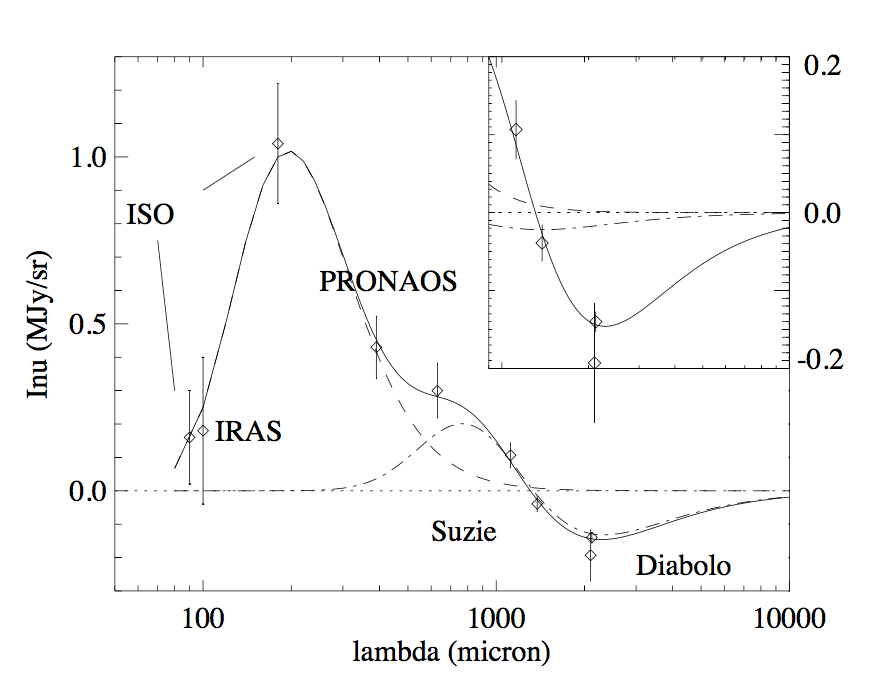
\includegraphics[width=0.5\textwidth]{birkinshaw1.png}
   \end{center}
\caption[TIME's frequency window will be mostly free of dust emission contamination. -(\cite{Birkinshaw1999})]{Measurements of Abell 2163 from mm to far-IR by multiple instruments. The solid line is a best-fit model for combined dust emission and SZE. The dash-dotted line is tSZE, while the dashed line is the isolated dust contribution. The dust emission falls off completely after $\sim$ 1000 microns [\cite{Birkinshaw1999}].}
\label{fig:dust}
\end{wrapfigure}

Intrinsic to this frequency range is also the ability to isolate the kSZE signal to high significance. In the left graph of Figure \ref{fig:tksze}, it was shown that for most frequencies, the kSZE signal is so faint that it is virtually impossible to detect for a high redshift cluster, if the tSZE signal is present. If the Kompaneets Equation presented above is examined more carefully, it can be seen that the tSZE has a null at 218 GHz, directly in the spectral range of TIME. This value can shift slightly for clusters with large numbers of relativistic electrons, as shown in the right graph of Figure \ref{fig:tksze}, but the effect is minimal. 

This combination of features allows for high significance kSZE measurements, without the explicit need for extremely high mass clusters, and without tSZE contamination.The expected measurements of kSZE for TIME are shown in Figure \ref{fig:time1}. TIME's sensitivity will easily reach kSZE intensities for a massive cluster at $v_{pec} = 1000 km/s$, and extend to clusters below that velocity.

\begin{figure}[h!]
\centering
\captionsetup{width=0.8\textwidth}
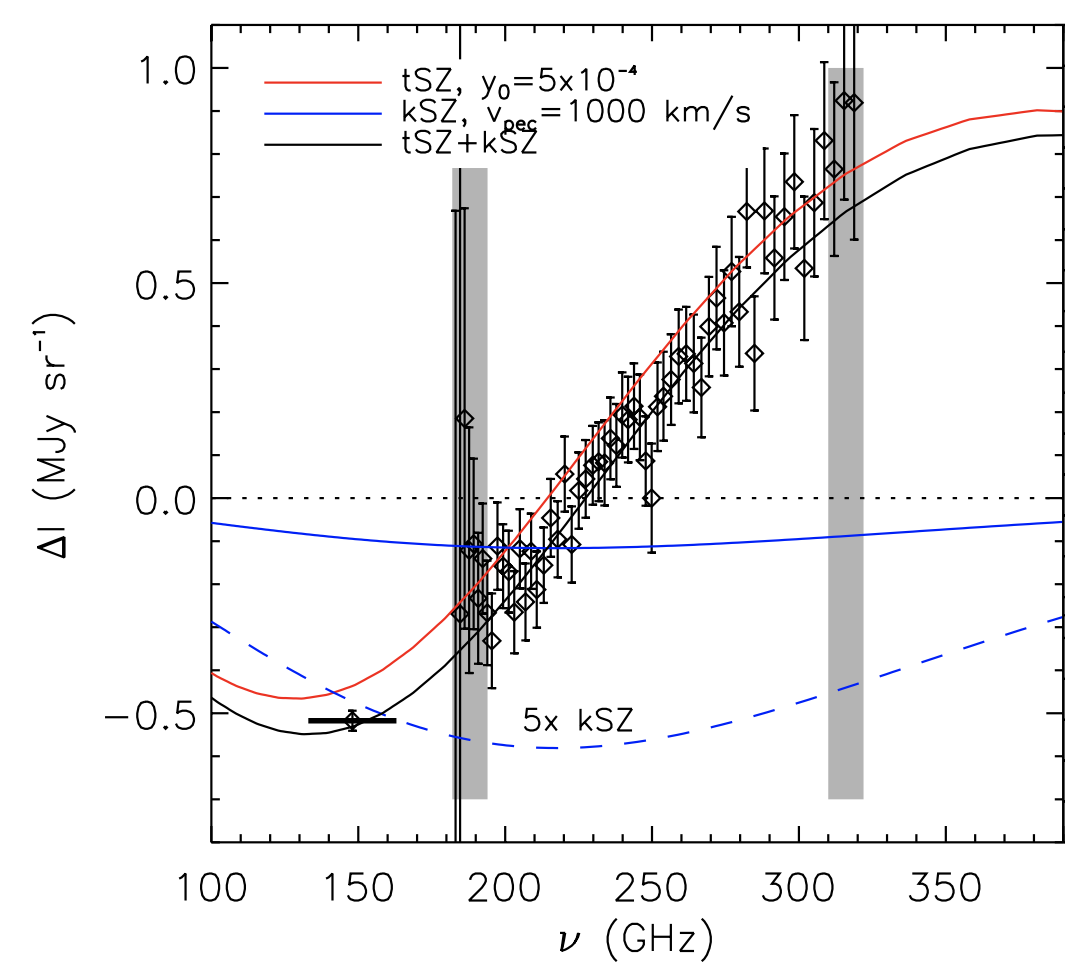
\includegraphics[width=0.8\textwidth]{time1.png}
\caption[Expected TIME kSZE & tSZE Measurements]{Simulated measurements of tSZE and kSZE with TIME. Grey bands are atmospheric monitoring channels. The solid and dashed lines are theoretical calculations of the effect using the equations given in the science discussion above, while the diamonds are the estimated performance for TIME. This estimated detection assumes astrophysical contamination, the atmospheric subtraction method described above, and assumes 10 hours of observation on the cluster.}
\label{fig:time1}
\end{figure}

%%%%%%%%%%%%%%%%%%%%%%%%%%%%%%%%%%%%%%%%%%%%%%%%%%%%%%%%%%%%%%%%%%%%%%%%%%%%%%%%%%
\section{TIME Instrument}

\begin{center}
    \begin{tabular}{|c|c|}
    \hline
     \multicolumn{2}{|c|}{TIME Experiment Parameters} \\
     \hline
     \hline
      Number of Spectrometers & 32: 16 each pol, grid diplexed \\
      Number of 150 GHz photometers   & 11, spectrally diplexed at 2 $f\lambda$ spacing \\
      Total Num of Detectors & 1920 + 11 = 1931: TES Bolometers with SQUID MUX \\
      Instantaneous FOV (ARO 12m) & 14 arcmin x 0.43 arcmin (mid-band) \\
      Cryostat, Base Temp & Existing 4K / 1K system w/ Helium cooler at 250 mK \\
      CII Survey Volume & 153 Mpc x 1.1 Mpc x 1240 Mpc deep \\
      CII Survey Integration Time & 1000 hours \\
      kSZ Peculiar Velocity Sensitivity & $\pm 1000 km/s$ per beam in 10 hours \\
      \hline
    \end{tabular}
\end{center}

\begin{center}
    \begin{tabular}{|c|c|c|c|}
    \hline
    \multicolumn{4}{|c|}{TIME Instrument Parameters} \\
    \hline
    \hline
    Parameter & Photometers & Grating LF Band & Grating HF Band \\
    \hline
    Spectral Range [GHz] & 135-165 & 183-230 & 230-326 \\
    Estimated end-to-end optical efficiency & 0.3 & 0.3 & 0.3 \\
    Num of Bolometers per sub-band & 1 & 24 (8x3) & 36 (12x3) \\
    Atmospheric PWV Monitor Channels & & 10: 183-199 GHz & 6: 305-326 GHz \\
    Frequency Resolution per Detector & 5 & 92-122 & 90-120 \\
    NEI on sky per detector [(MJy/sr)$\sqrt{s}$] & 0.44 & 4.7-5.8 & 7.3-15.2 \\
    NEFD on sky per detector [mJy$\sqrt{s}$] & 6.7 & 84-105 & 101-131 \\
    \hline
    \end{tabular}
\end{center}

\begin{center}
    \begin{tabular}{|c|c|c|c|}
    \hline
    \multicolumn{4}{|c|}{TES Bolometer Parameters} \\
    \hline
    \hline
    Parameter & Photometers & Grating LF Band & Grating HF Band \\
    \hline
    TES safety factor ($P_{elec}/P_{opt}$) & 2.5 & 2.4-2.8 & 2.1-5.1 \\
    Detector + MUX NEP [$10^{-18} W Hz^{-1/2}$] & 40 & 9.7 & 13 \\
    Photon NEP [$10^{-18} W Hz^{-1/2}$] & 60 & 23-26 & 26-43 \\
    Absorber Size [mm] & 4.0 & 3.0 x 3.48 & 3.0 x 2.32 \\
    \hline 
    \end{tabular}
\end{center}
\subsection{Detector Characteristics}

The TIME instrument will have an instantaneous field of view of 11 x 0.35 arcminutes split into a 16 x 1 series of spatial pixels. This wide field is made possible by two banks of curved grating spectrometers, each of which can handle a single polarization, and with an R = 100 resolution (see Figure ~\ref{fig:jon2}). Within are parallel-plate waveguides which both focus and diffract light from a single feedhorn to the array of 60 transition edge sensor (TES) bolometers. This unique design drastically reduces the weight and volume of the spectrometer compared to devices used in similar instruments. Combined, the two banks will store 1920 total detectors divided into 6 blocks, and covering 8-12 spectral pixels. The total expected spectral coverage will range from 183-326 GHz, with each channel width at 2-3 GHz, and added edge channels for atmospheric noise reduction [\cite{Crites2014},\cite{Hunacek2016}].

The detectors are biased through superconducting flex cables by NIST Superconducting Quantum Interference Devices (SQUIDS), which have low noise, low power dissipation, and a low impedance, making them the ideal pre-amplifier for TES bolometers [\cite{Dobbs2009}]. Time domain multiplexing allows the SQUIDS to bias multiple detectors through a single set of cables simultaneously. The detectors are then read out with a Multi-Channel Electronics system designed by UBC [\cite{Battistelli2008}].

The entire instrument is housed in a closed cycle cryostat with 5 stages ranging from 50 K, using pulse tube refrigeration, down to the base temperature of 250 mK, utilizing 3He sorption. The cryostat is shown below in Figure ~\ref{fig:jon1}

\begin{figure}[h!]
\centering
\captionsetup{width=0.8\textwidth}
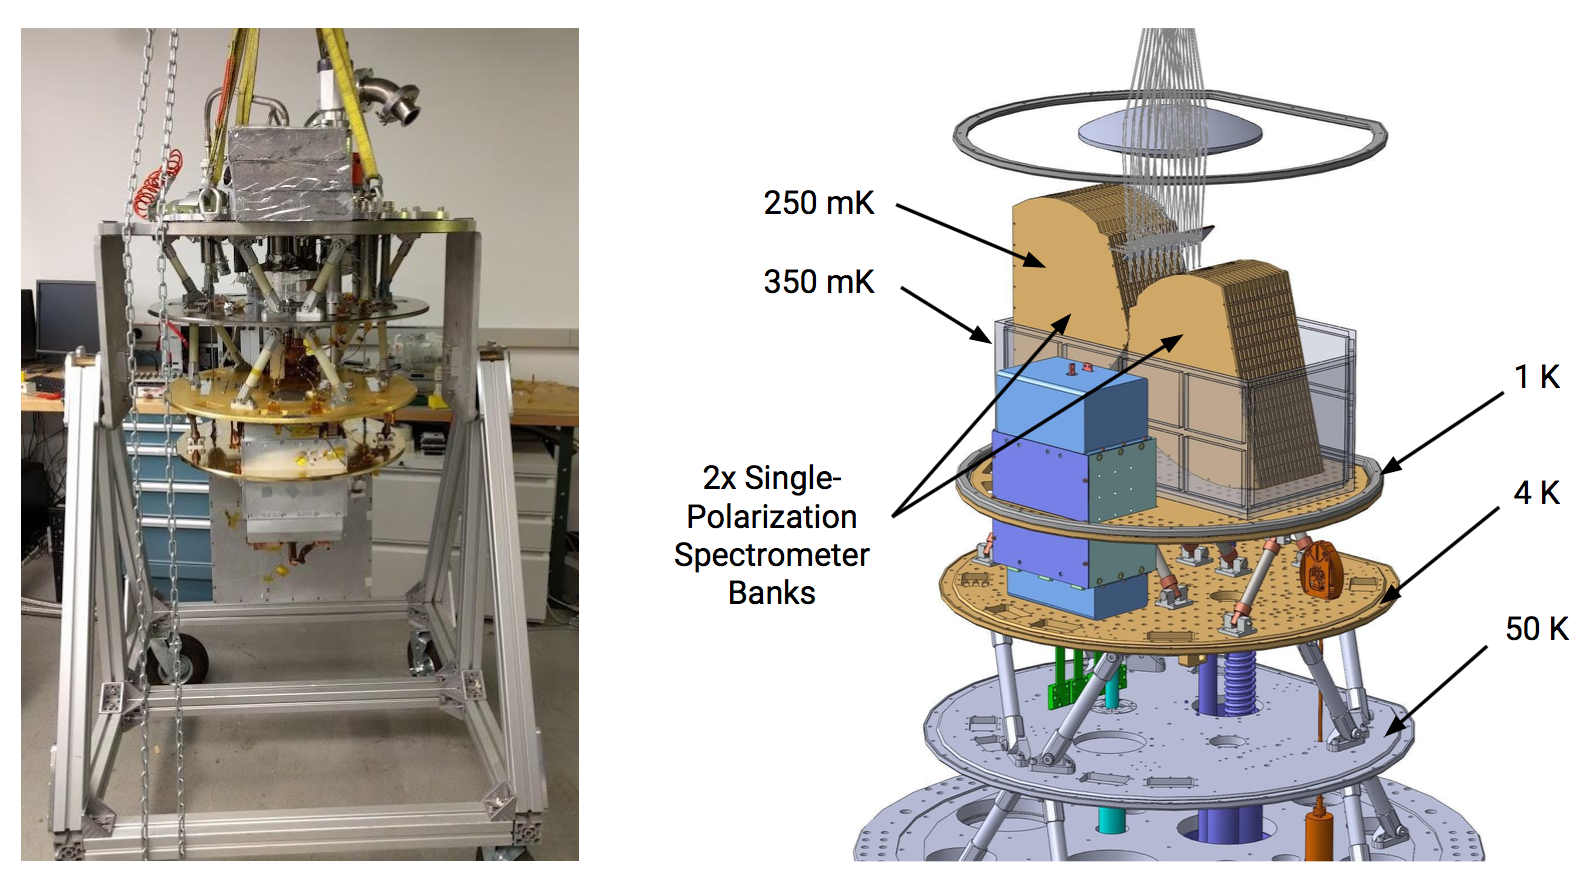
\includegraphics[width=0.8\textwidth]{jon1.png}
\caption[TIME Cryostat -[\cite{Hunacek2016}]]{Left: Cryostat on support structure without shields. Right: Model of Cryostat showing placement of the spectrometer banks. [\cite{Hunacek2016}]}
\label{fig:jon1}
\end{figure}

\begin{figure}[h!]
\centering
\captionsetup{width=0.8\textwidth}
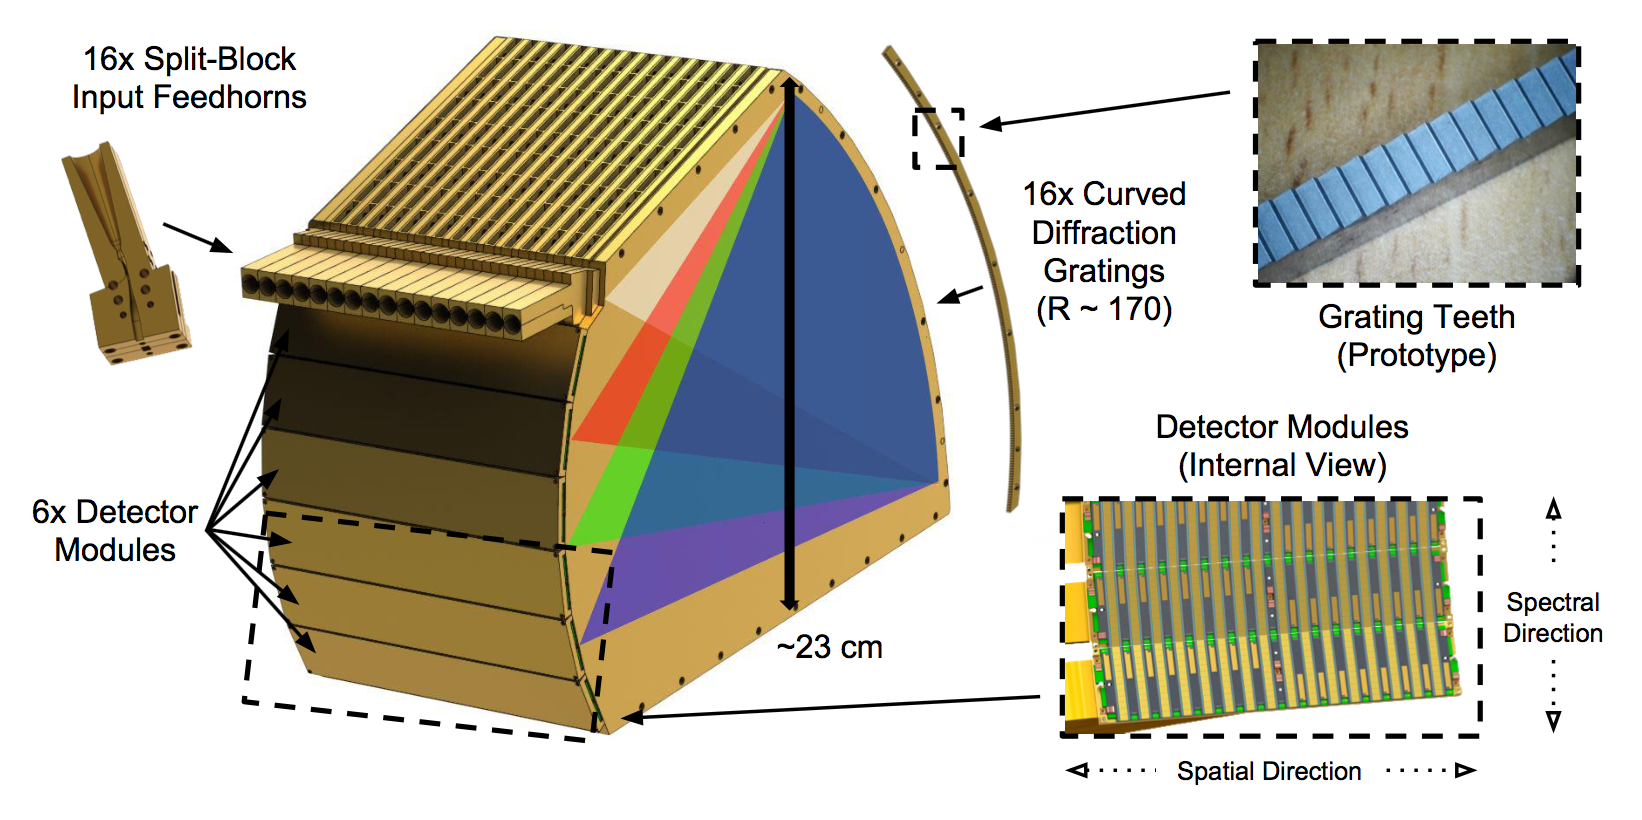
\includegraphics[width=0.8\textwidth]{jon2.png}
\caption[TIME Spectrometer Banks and Detector Modules -[\cite{Hunacek2016}]]{TIME closed-cycle cryostat [\cite{Hunacek2016}]}
\label{fig:jon2}
\end{figure}

\subsection{Observation Strategy}

TIME is utilizing grating spectrometers that are capable of rendering not only spectral but also spatial information into a 3 dimensional data cube. This adds the benefit of separating a superposition of signals from different redshifts along the line of sight, but in the same spatial pixel. For research on the CMB and the EOR, this is an especially useful tool as it allows both foreground and background sources to be individually measured. In the case of TIME, this implies the ability to distinguish between the faint dwarf galaxy population of interest and the much brighter foreground galaxies. 
Complementary to the spectrometers, the chosen observing method will have the ability to constrain faint CO and CII line emission at high redshift though intensity mapping. This is a tested technique [\cite{Keating2015},\cite{Keating2016}] accomplished by moving the array of detectors across the sky, and recording the spatial variation in the total surface brightness from all sources, as bolometer arrays are sensitive to the integrated intensity. Traditional measurements of faint galaxies attempt to resolve a single source through interferometry, such as with the Atacama Large Millimeter Array (ALMA), but typically miss the faintest end of the full luminosity function. With intensity mapping, lower limits on the faint end of the function can be determined, using only a single dish, rather than an entire array. Compared to ALMA, which would take roughly 4500 hours to observe a 2.5 degree field of view [\cite{Kovetz2017}], TIME can scan that same area in 1000 hours. 

TIME will be commissioned at the Arizona Radio Observatory (ARO) at Kitt Peak on the 12 meter ALMA Prototype Antenna. Once there it will undergo a series of tests and calibrations, and will eventually start observations. It will be completing constant declination scans of several individual clusters by rastering back and forth across the source. An example scan pattern is shown in Figure ~\ref{fig:time2ab}  and ~\ref{fig:time2cd} below. The ideal strategy will be to scan two 1.3 degree linear fields over the course of 9 hours for CII/CO, and further dedicated time for kSZ detection in selected galaxy clusters.

\begin{figure}[!ht]%
    \centering
    \subfloat{{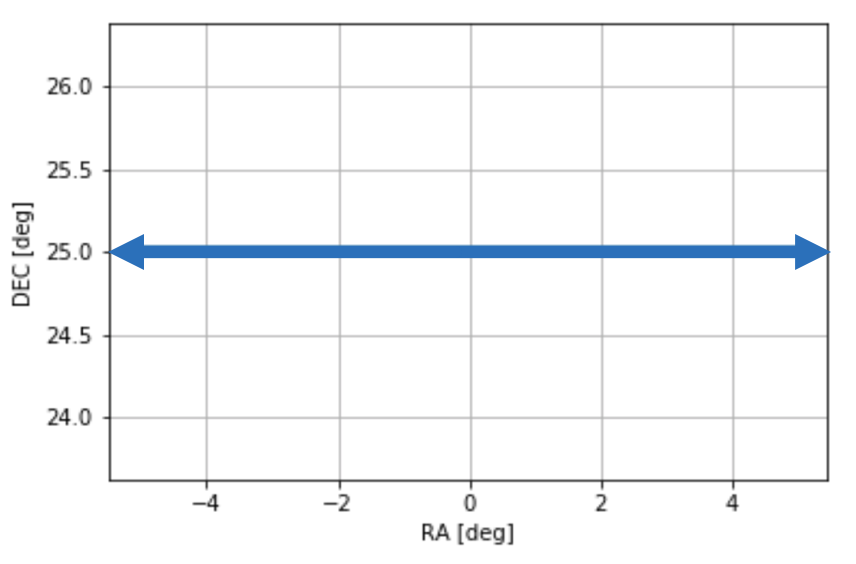
\includegraphics[width=0.45\textwidth]{time2a.png} }}%
    \qquad
    \subfloat{{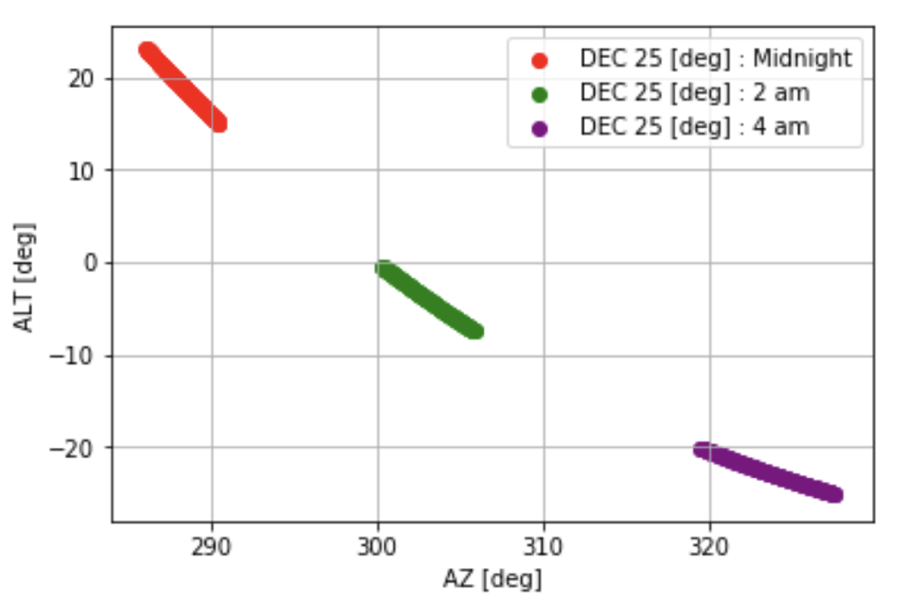
\includegraphics[width=0.45\textwidth]{time2b.png} }}%
    \singlespace
    \caption[]{}%
    \label{fig:time2ab}%
\end{figure}

\begin{figure}[!ht]%
    \centering
    \subfloat{{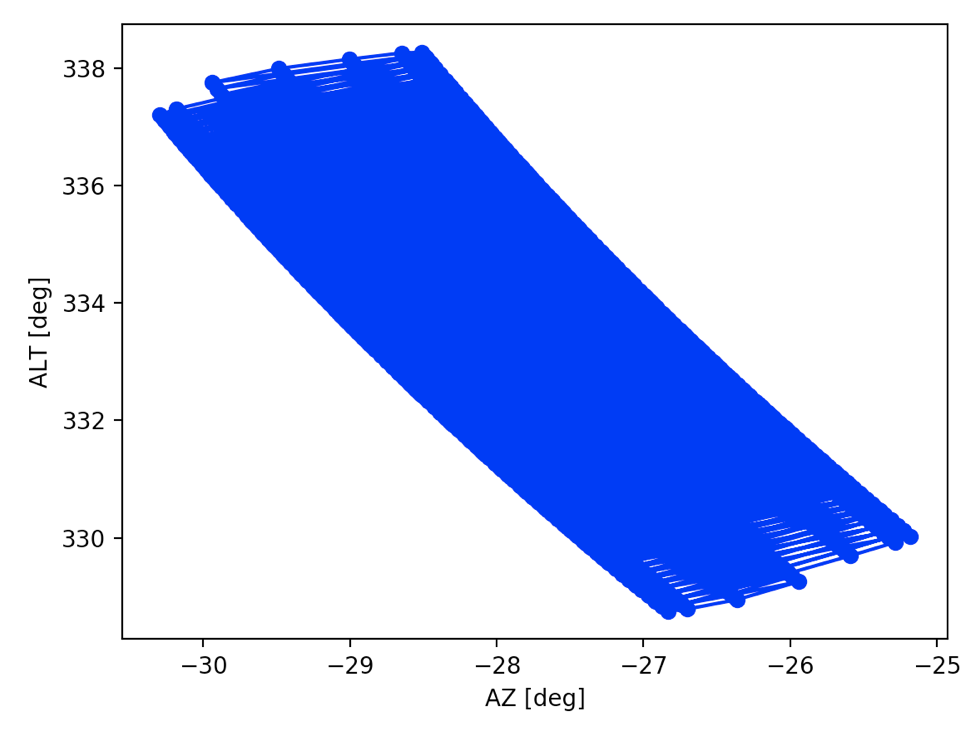
\includegraphics[width=0.45\textwidth]{time2c.png} }}%
    \qquad
    \subfloat{{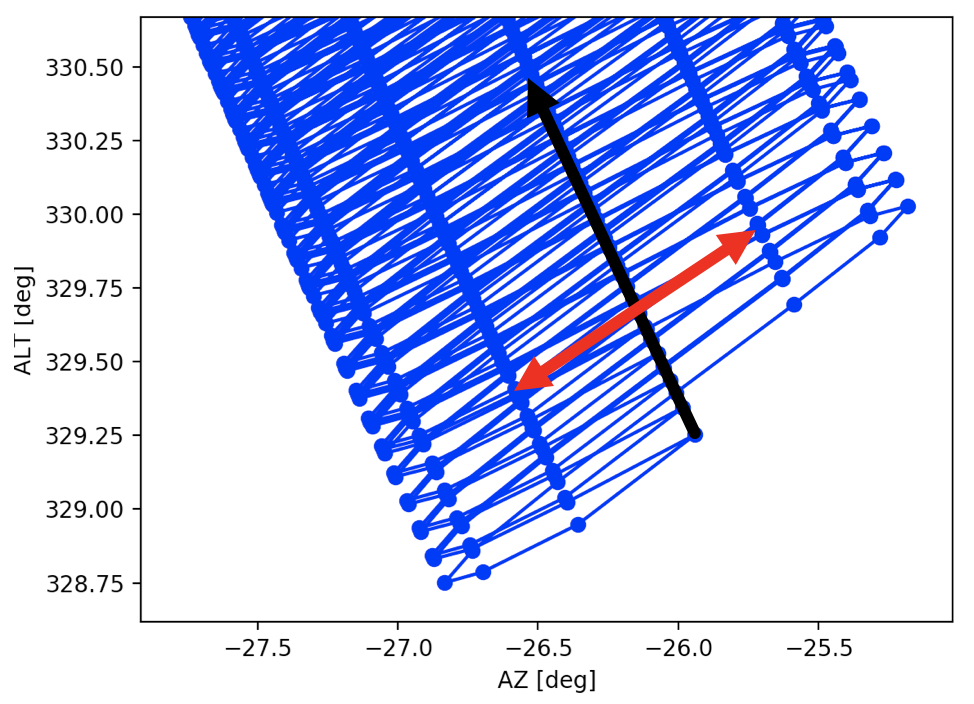
\includegraphics[width=0.45\textwidth]{time2d.png} }}%
    \singlespace
    \caption[]{}%
    \label{fig:time2ab}%
\end{figure}

%%%%%%%%%%%%%%%%%%%%%%%%%%%%%%%%%%%%%%%%%%%%%%%%%%%%%%%%%%%%%%%%%%%%%%%%%%%%%%%%%%
\section{TIME Software Development}

In order to facilitate the successful completion of the TIME scientific goals, an important consideration is the handling of data and intercommunication between devices.
\begin{wrapfigure}{r}{0.5\textwidth}
\vspace{-0.8cm}
  \begin{center}
    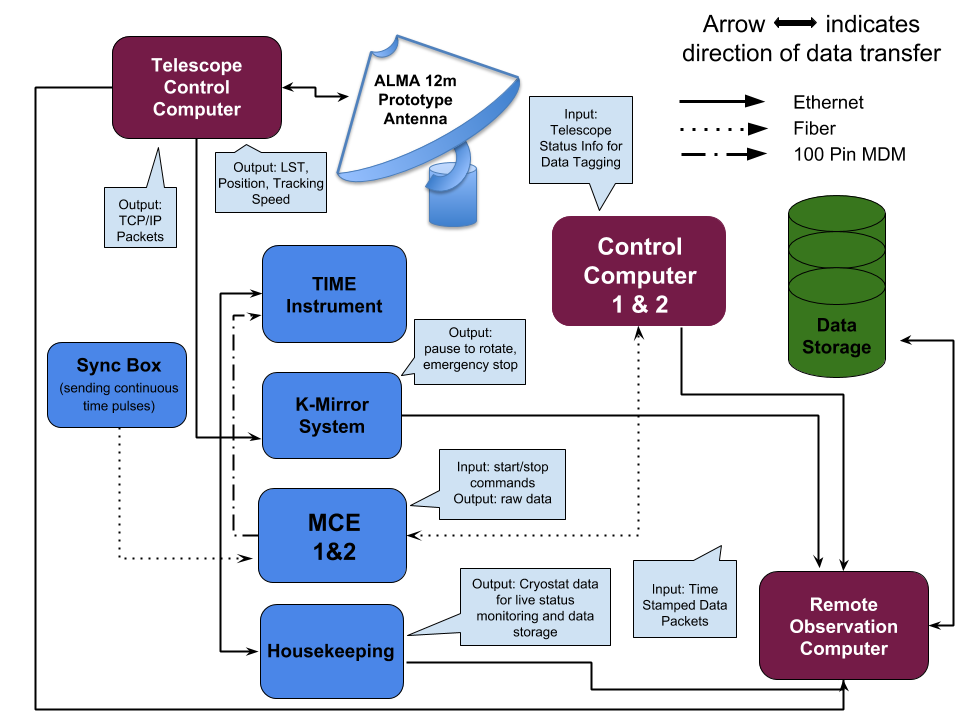
\includegraphics[width=0.55\textwidth]{km9.png}
  \end{center}
  \caption[TIME Control Flow Diagram]{Communications layout for TIME. Each instrument in blue represents a source of data, some of which will pass through the Control Computer, onto the Remote Observing Computer, and finally into Data Storage. There will be two MCEs each with their own control computer, a telescope computer, and a Raspberry Pi 3 controlling the K-Mirror. Each of those systems will send output to the Remote Observing Computer running the GUI over SSH and SFTP protocols. All data will then be stored in multiple locations, including the remote computer, an external hard drive, and stored in a cloud.}
  \label{fig:km9}
\end{wrapfigure}
 A schematic of the hardware layout and connections is included in Figure ~\ref{fig:km9}, which details the communication pathways for multiple devices, including the telescope, control computer, Multi Channel Electronics (MCE), K-Mirror, and others. The key to successful data acquisition will be synchronous operation of each system, and eventual data collation. One of the most difficult problems is how to collate the many different ``clocks'' in the schematic into one universal standard time that is placed into the permanent data files. The most sensitive connection is the one between the MCE and telescope, since positional location over a source must correspond directly to a signal received and transmitted from the MCE. In an example scenario of a scan across a cluster for CII detection, if the telescope pointing information were to have some sort of lag relative to the bolometer signal, the final analysis would result in a cluster that appeared to be have a higher fraction of CII present in the outskirts than was predicted by modeling. This could lead to an assumption of physical properties for that cluster that are inaccurate. 
 
The solution to this problem is two-fold. The first requires the MCE to have an independent time source. The MCE currently has a device known as a sync box, which sends 25 MHz 32-bit sequential steps that are encoded into each data frame. When both MCE's are run, the sync box ensures that these stamps are placed on the same frame (i.e. both first frames would have the same sequential number), allowing files to be compared during collation. The second involves a configuration of the hardware which produces Data Valid pulses based on an external trigger. The trigger planned for use with TIME will be an N2X system, which is slaved over a Network Time Protocol (NTP) to UTC time in seconds. NTP is a standard time keeping server that simulates an atomic clock and kept accurate with GPS. The device is then configured to produce the exact same number of pulses in between each UTC second. Since the telescope also understands UTC time, the time at frame generation by the MCE can be compared with location of the telescope at that same time without fear of lag. This implementation has yet to be tested, however the sync box has already been integrated into the system and produces the expected behavior. 

Integration of the other components will simply be a matter of data transfer over the local network available at the telescope, processed through a script on the remote observing computer, and then finally stored in multiple locations. The functionality of the software and the description of this process is provided below. 


\subsection{Graphical User Interface}

For lab testing and on-site live data visualization, a graphical user interface (GUI) was designed in a {\sc Python} script, and initially implemented in a web based framework using {\sc Dash by Plotly}. The GUI acts like a HUB, with input and output to multiple devices which all show statuses on the screen. Currently added functions include viewing the data from the MCE, with both live and archival data, a heatmap of the detector channels, and simulated inputs from the K-mirror and telescope. Figures ~\ref{fig:gui1} and ~\ref{fig:gui2} show the first and second iterations of the GUI. In the first iteration, the MCE was activated by a python script, the incoming data was parsed by another script and fed to the Plotly servers, and then a separate script stored the data in a preferred format. A web browser could then be opened and sent to a local host address where the user could view and interact with the data. This version was abandoned after testing the MCE at the highest data rate of 400 Hz, with 2 seconds of data on the screen at a time, updates every 1 second, and run for 8 hours. At this data rate, the MCE generates 374 frames per second. When looking at the output for only one detector, 374 data points are added to the screen per second, with over 12,000 data points present in every array. When run for an extended time, the lag on screen became visibly noticeable, as it would take longer and longer for the graphs to update, and some frames were even skipped entirely. This was due to the method by which Plotly updated its streaming plots, where it would have to re-draw every data point every time the graphs were refreshed, meaning that after 30 seconds, 11,000 data points were on the screen at a time. For lab testing, it was necessary to have at least 2 minutes of data on the screen at one time.

\begin{figure}[ht!]
	\centering
	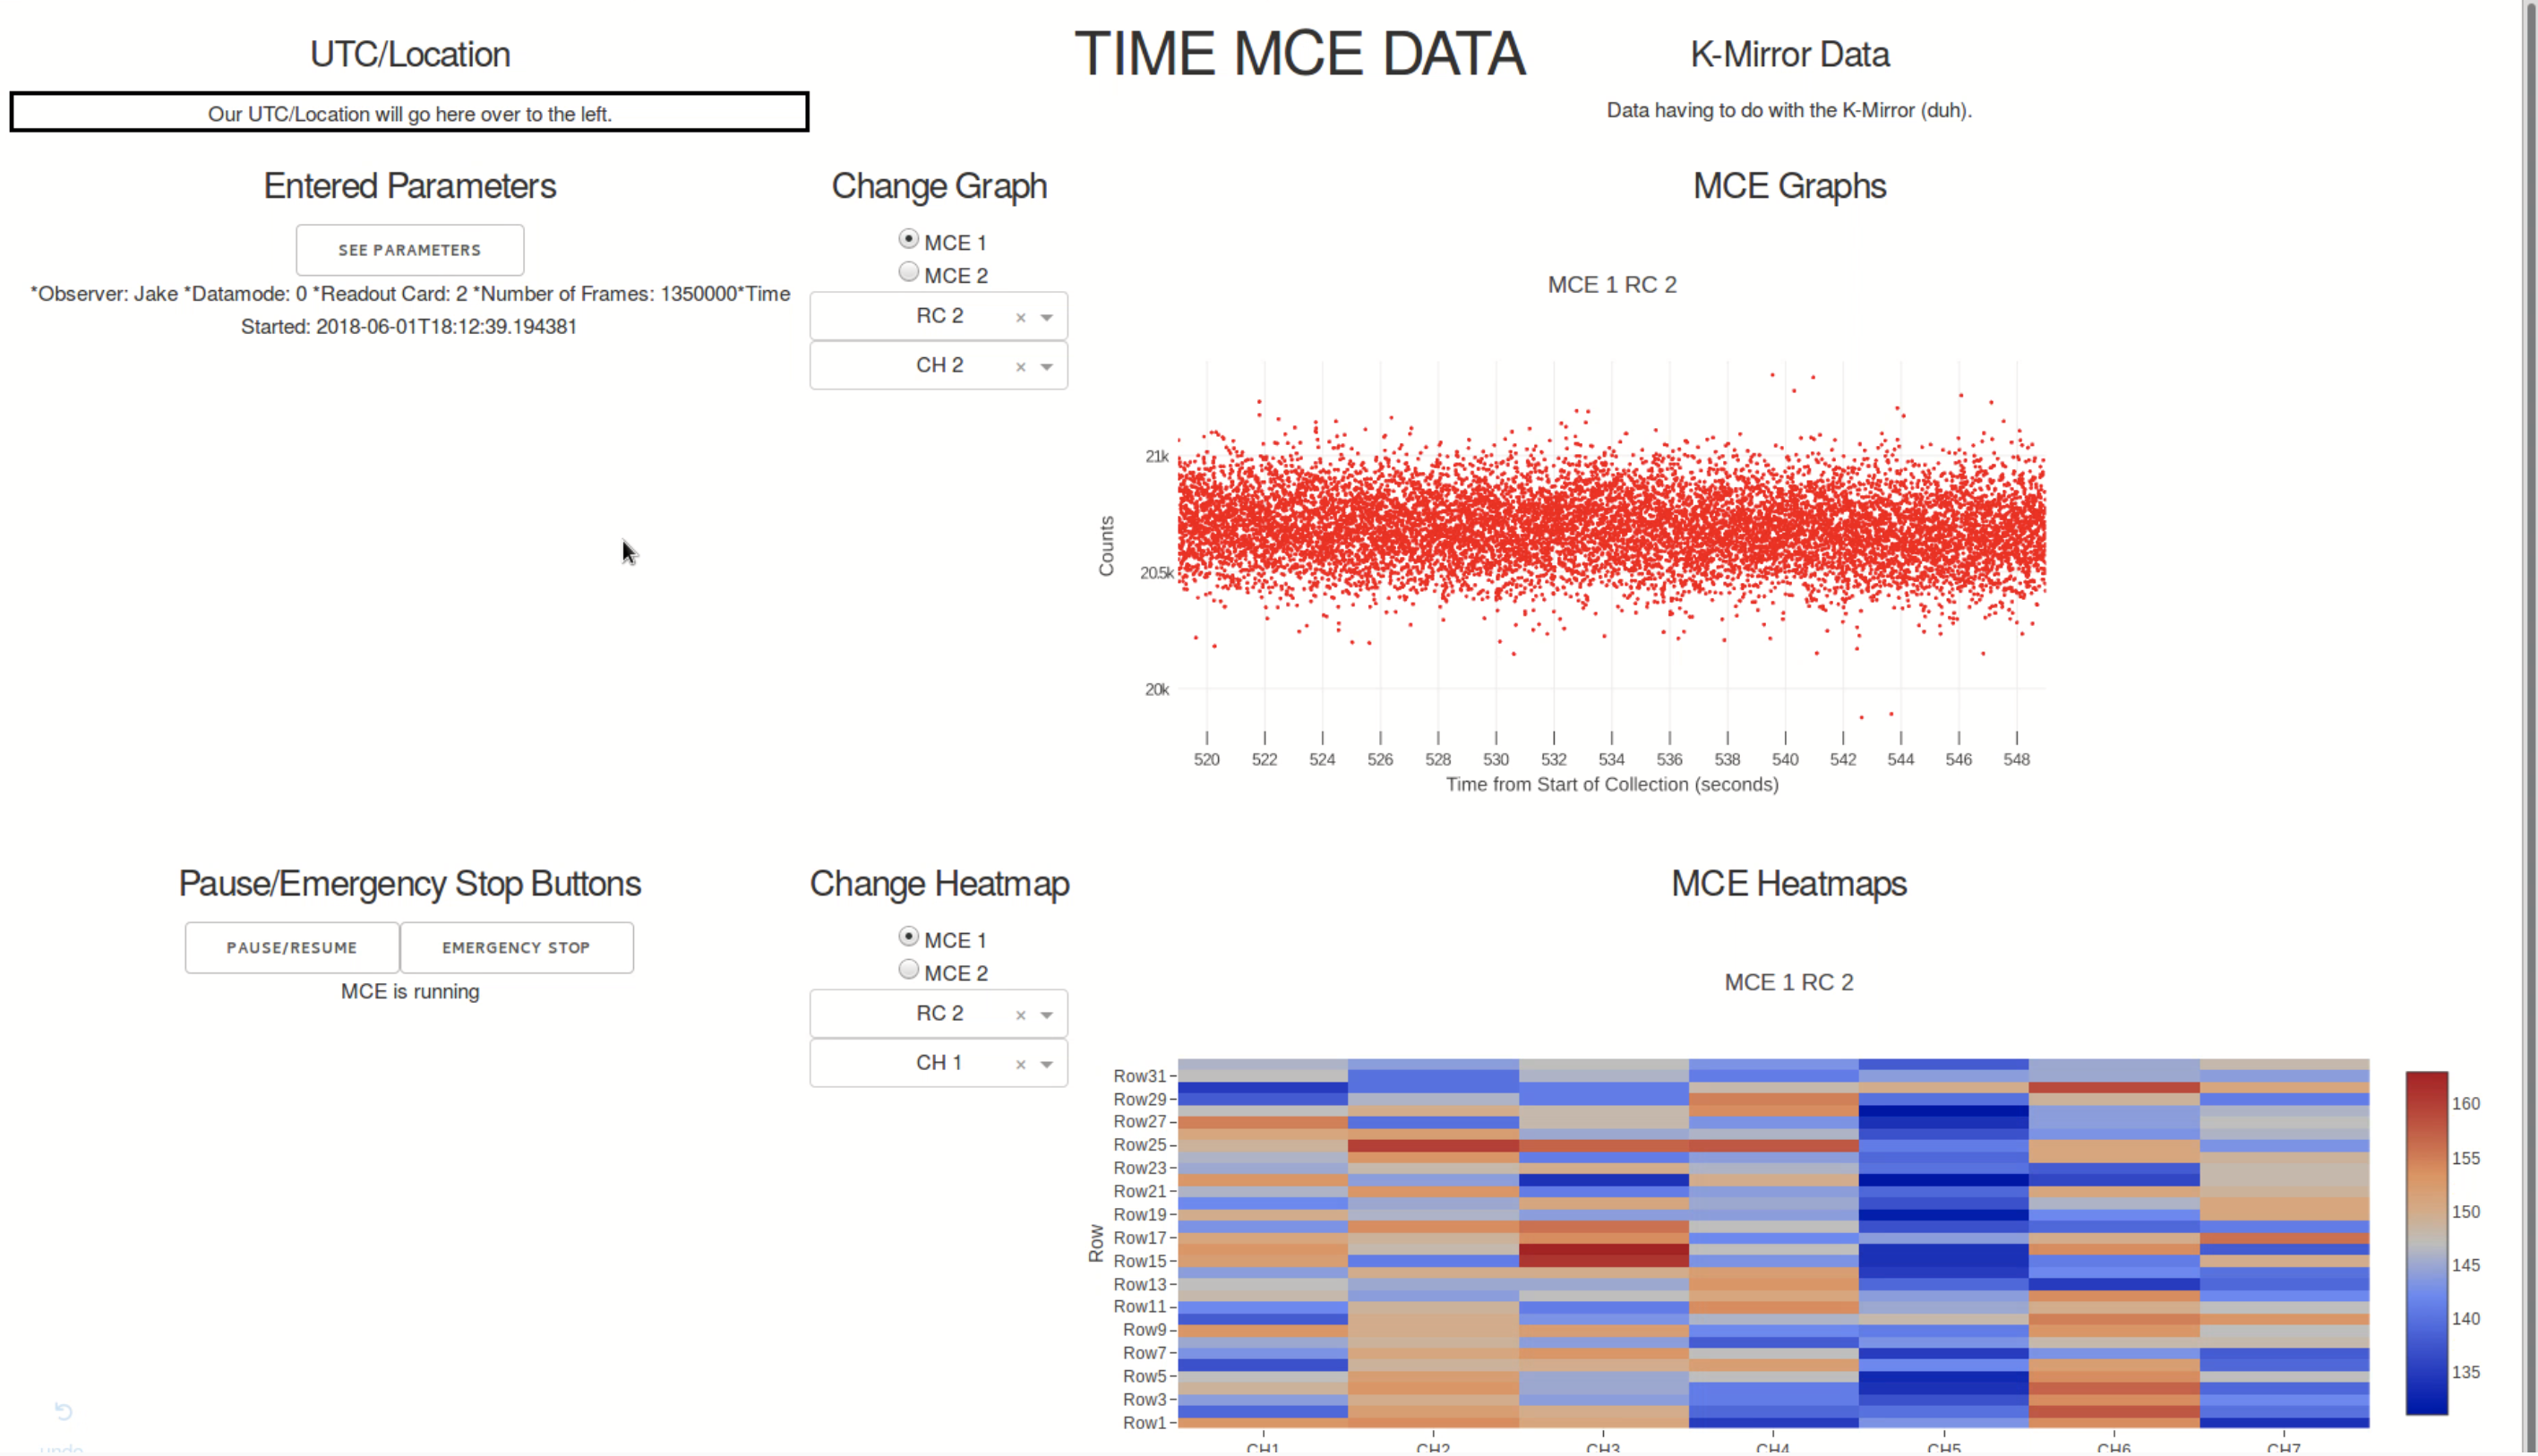
\includegraphics[width=\textwidth]{gui1.png}%
	\caption[GUI Beta 1.0]{}%
	\label{fig:gui1}%
\end{figure}

\begin{figure}[ht!]
	\centering
	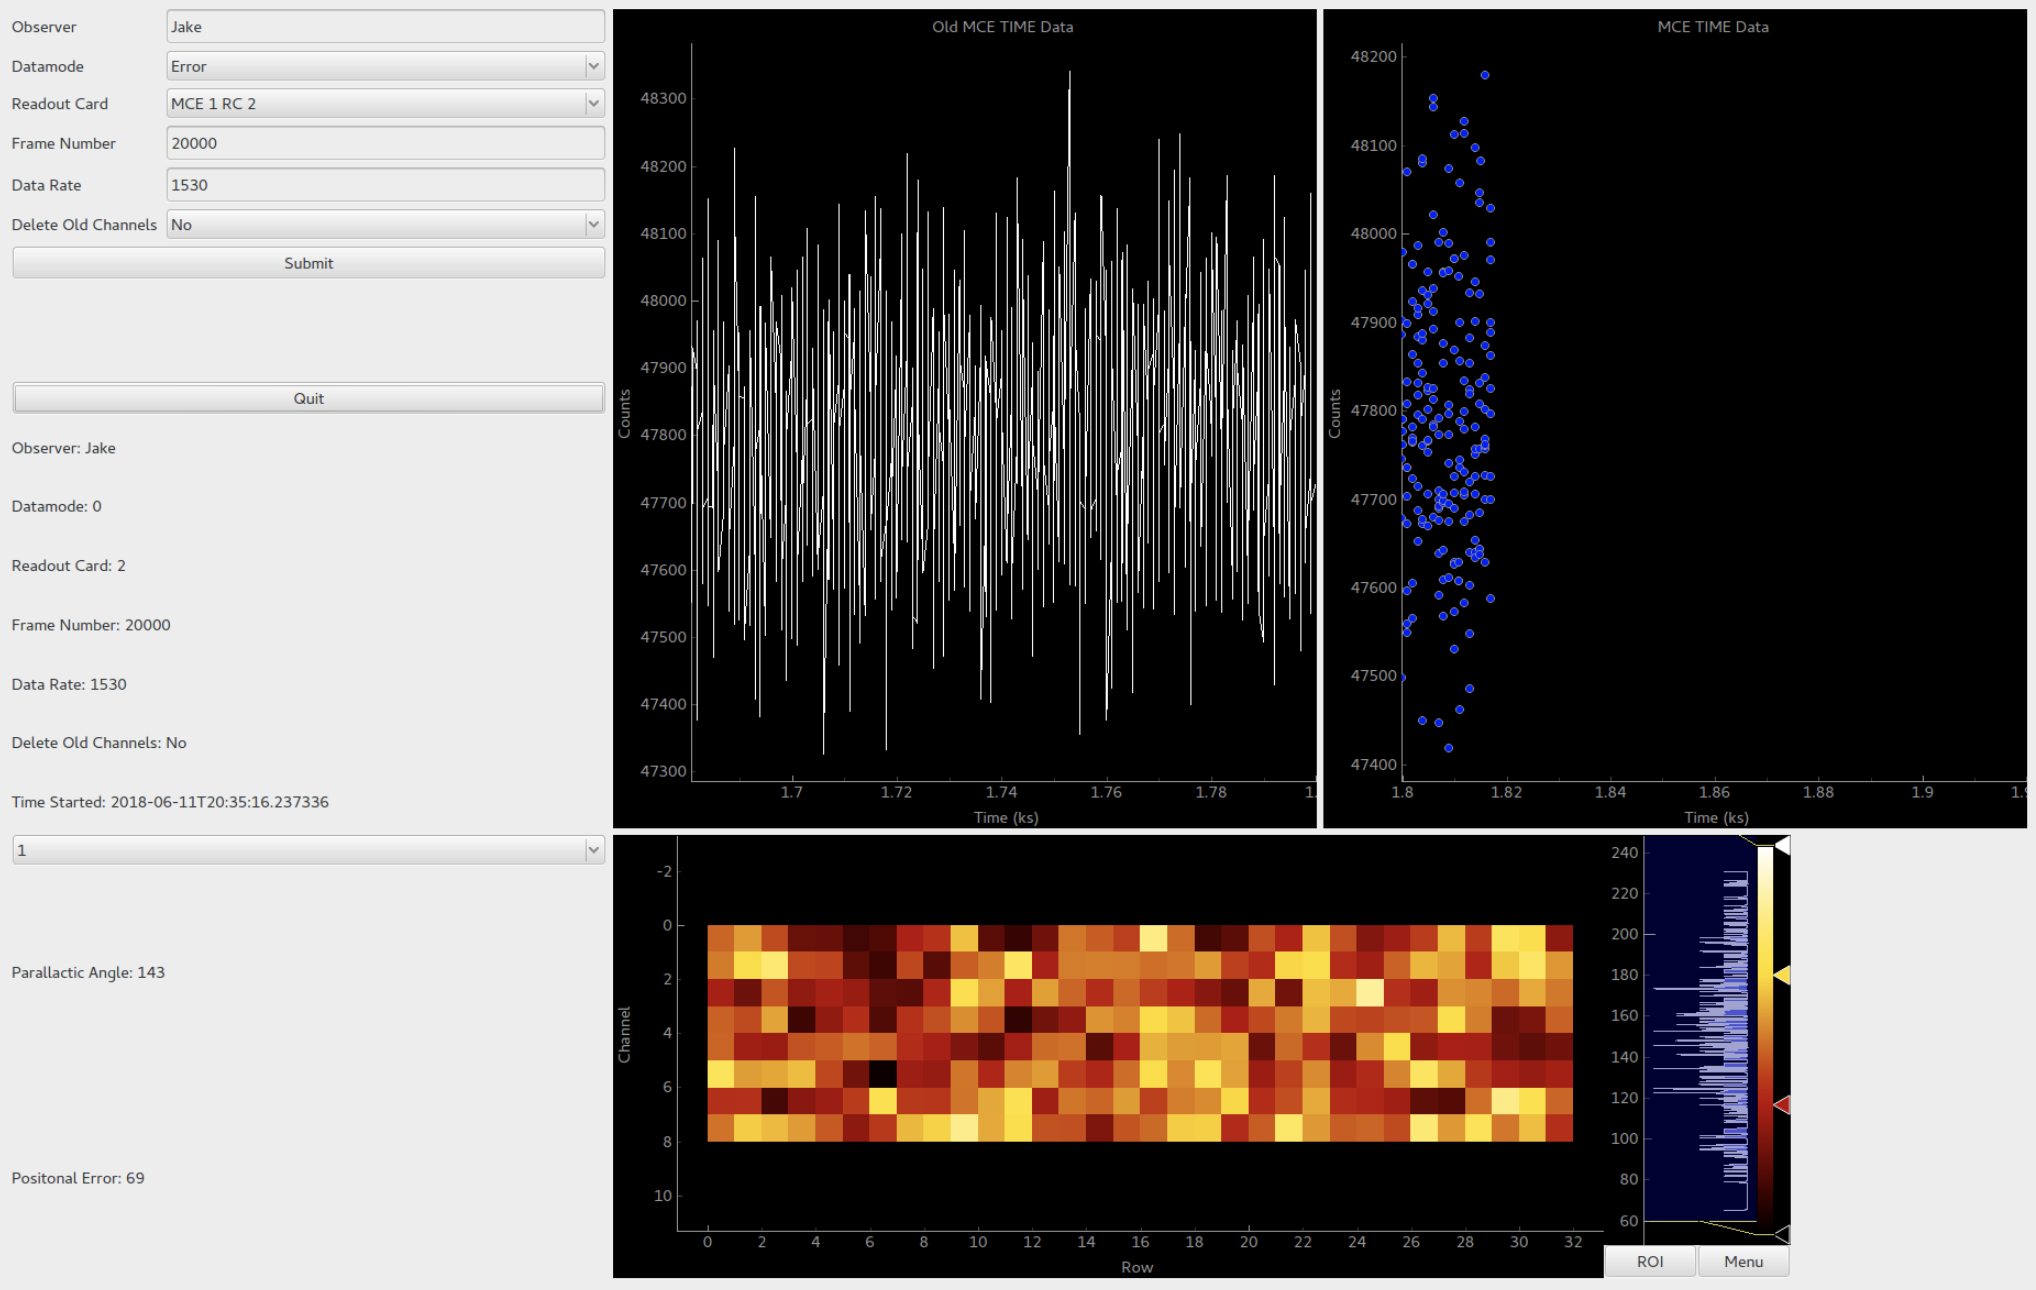
\includegraphics[width=\textwidth]{gui2.png}%
	\caption[GUI Beta 2.0]{}%
	\label{fig:gui2}%
\end{figure}

The second version of the GUI was created using PyQt4 graphics packages and required a re-write from the html based script employed before. This script only updated the graphs with the newest data, without redrawing the whole figure, and wasn't subject to the unpredictability of web servers. The necessary packages could also simply be downloaded through ``apt-get'' from a standard library and added to the users existing python library. This new system was tested using the same parameters as the first, which revealed only one minor flaw. The parameters for the MCE input by the user, including data rate, would return a frame per second that would not be an integer value. At a data rate of 45, the value was exactly 374 frames per second, but at a data rate of 10, it was 1683.5 frames per second. This meant that every other second, an extra file was created, and missed by the previous check by the software. This was easily corrected for by adding in a check for an extra file that would be parsed and incorporated onscreen in the correct chronological order. After testing the system with 5 minutes of data onscreen at a time for 8 hours, there were no lags to the system. 

Items that must still be incorporated into the GUI are actual interfacing from the K-Mirror and the Telescope. A telescope simulator was created to mimic the observing patterns required for TIME (constant declination scans) which outputs positional information and other metrics necessary for the K-Mirror operation described in detail later. The next step in testing will involve data generation from these simulated sources, transferred over SSH, and then visualized on the remote observing computer. 

\subsection{Data Storage}

Data storage is a challenge for every scientific mission, and no less so for TIME. With 2 MCEs collecting 50 MHz data, telescope data at 20 packets/second, and numerous other electronics, the sheer volume and speed at which data sets develop requires very specific packaging solutions. 

%One problem is how to collate the data so that it is time sequenced synchronously across each output. The telescope computer has an internal clock, as does the K-Mirror computer and the control computer. But due to the finite nature of data transfer and manipulation, by the time each stream is collected into the remote observing computer, each can be seconds apart from one another. The importance of this flaw is easily seen from a case where corrupted data is removed based on error flags, or problems with the detectors. If data is removed based on the time at which the flag was triggered, but there is a delay between when the control computer reads that flag and commands the telescope to stop tracking, then the two different instances will be recorded as disparate events in the data file, and more data will be deleted than necessary. The solution to this problem is to create a unifying time keeper that will continuously send time ``pulses'' to the control computer, and where it can be appropriately used to tag any information that passes through the hub. For the two MCEs, this device already exists in the form of a ``sync box'', which ensures that both MCE's are acquiring frames and are recording the timestamps synchronously. While this feature has been tested on previous experiments such as BICEP2, integrating it with the control computer and the other components could be complicated. The K-Mirror, for example, is not designed to take a fiber optic input, and the sync box connection has not been tested on anything other than a computer with the MCE control system installed. An alternative solution is to use the Telescope control computer. Information flows out of it and into the control computer and the K-Mirror system. Every other hardware device data stream is collected at the control computer and can be stamped with the telescope time upon storage. This would be ideal since the control computer will be on site at Kitt Peak, and directly connected to the local server. Any lag induced by the transfer would be minimal, and the telescope UTC time is rated accurate to other world clocks to within microseconds. 
%

The best file system is one that can both be flexible about the type of data (int, string, bool, float), and also the way that it can be packaged and recalled. Several formats were considered including Dirfiles, NetCDF, HDF5, FITS, and custom binaries, because they could all be integrated into Python scripts. Dirfiles are the natural file format for the MCE system which work extremely efficiently for time ordered data. However, there are other data types for which it might be an unnatural fit, such as K-Mirror status flags. It also can only be read out in a very specific way, which could be inhibitive to large data sets. FITS files are a natural choice for working with any sort of image array, but TIME bolometers are not a one to one analog for image data. There were no strong objections to using this method, other than it was outdated and not as efficient as other options. Custom binaries would have been useful, but they have very little documentation, and so the benefits and drawbacks were difficult to assess. In the end, the NetCDF4 file option was chosen for a number of reasons. It has an easy integration with Python, and is in fact built into the standard {\sc Anaconda} distribution, without the need to separately install any other supporting packages, such as HDF5 integration. It is also heavily documented, and used by a large variety of different fields. However, the most useful attributes include direct rather than sequential data access, and an unlimited file size (within system limitations). The ability to search for data directly removes the problem of files which are too large to parse. As an example, in python, a text file is read in line by line, with the readout time increasing with the number of lines. In a NetCDF4 file, data can be queried based on the parameters or attributes assigned to it. One parameter set by the TIME GUI is the observer. As such, a massive NetCDF file could be queried to only return data for a specific variable, over a set of times for only that observer. The entire file is not retrieved for the user, but is scanned by the software to look for the appropriate data to return. While these are perfect qualities for our system, the size of the file is still ideally kept to a small value, to facilitate easier transfer over ethernet connections. NetCDF allows the user to break up the data across multiple small files, but still read them back as if they were all the same file. So, if the observer happened to be on call for more than one night, all of the data pertaining to that observer would be called from multiple files. Lastly but not least is the flexibility of the underlying architecture for data storage. It operates similar to a python dictionary, where the user can create logical groupings and assign variables and dimensions with specific attributes. For the TIME GUI, MCE data is stored in three groups; gui parameters, raw data, and heatmap data. Each of these groups has their own set of variables and dimensions, with each variable being assigned an attribute. For the gui parameters, there is a variable called ``header'' which was given attributes ``mce frame header info'', and ``updated once per frame file'', and listing what data types and how much file memory it consumed. Other variables, such as heatmap data, could also have attributes stating what units the data were in. The attributes can be called by the user at any time to assist with recollection of what is contained in the variable. More usefully, attributes can also be added to the time ordered data in the form of flags. If the K-Mirror system malfunctions, it is set to send an error flag to the GUI, which can then be added as an attribute to data over the range of time that the error occurred. Later during data analysis, the attributes can be used to filter out contaminated data. 

\subsection{Higher Level Data Analysis Suite}

The software described above works well for situations in the lab for live visualization of the detector arrays. However, additional software is required for commissioning of the instrument, and actual observations. For the telescope, a number of tests are required to ensure that the pointing is accurate. This requires generation of 

%%%%%%%%%%%%%%%%%%%%%%%%%%%%%%%%%%%%%%%%%%%%%%%%%%%%%%%%%%%%%%%%%%%%%%%%%%%%%%%%%
\section{K-Mirror Image Rotator}
The telescope at which TIME will be deployed is an ALMA Prototype 12m antenna, with an Alt-Azimuth mount. 
\begin{wrapfigure}{r}{0.5\textwidth}
\vspace{-0.8cm}
  \begin{center}
    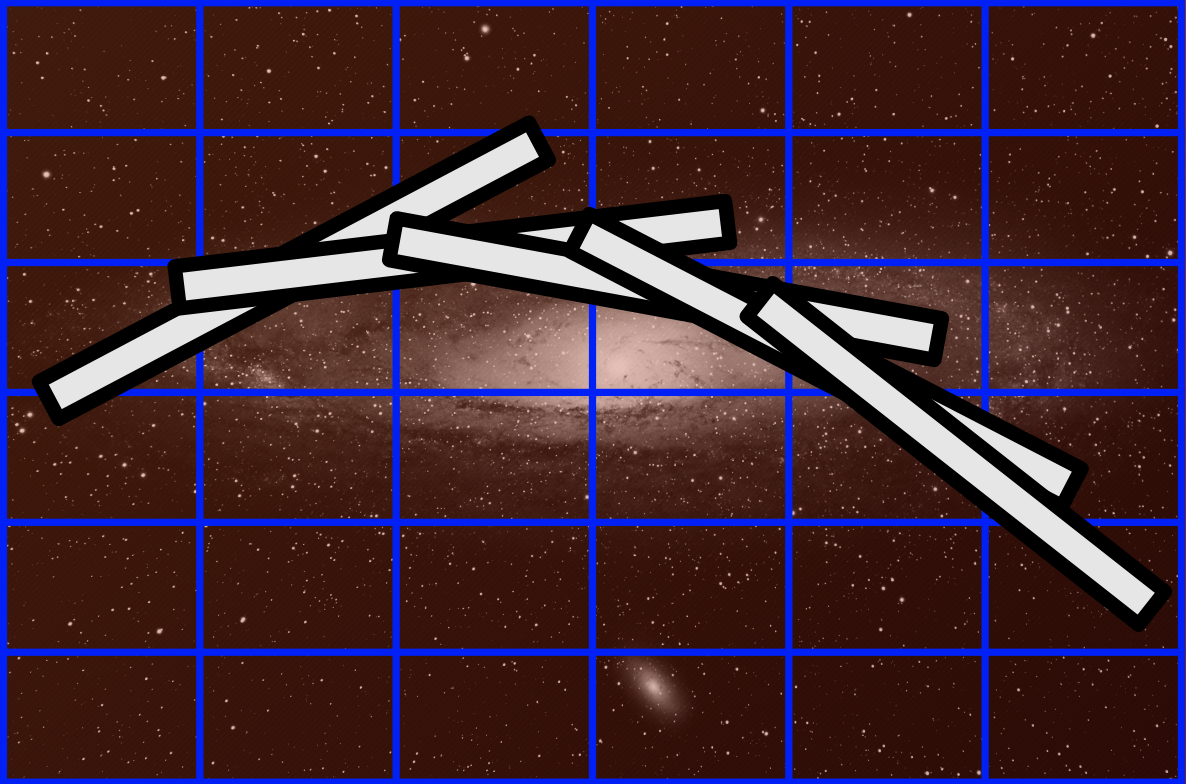
\includegraphics[width=0.48\textwidth]{km1.png}
  \end{center}
  \caption[Diagram of Bolometer De-rotation on Source from Alt-Az Mount.]{The white rectangles are a representation of the bolometer array projected on a galaxy source. As the galaxy naturally moves with time due to the earth's rotation, the line becomes rotated, causing overlapping regions and missing pixels. When the telescope moves to keep itself centered on the source, this problem would become more pronounced. For KSZ measurements, the resulting data would show extremely high thermal measurements in the centers of clusters, and almost none on the outskirts.}
  \label{fig:km1}
\end{wrapfigure}
This presents unique challenges for the optical path from the primary mirror to the cryostat, because of the line scan observation strategy. The reason why can be easily shown in Figure ~\ref{fig:km1}. The rotation of the earth causes objects on the sky to trace out a circular path with time, while the telescope mount provides motion only in linear directions, not circularly. When the line of bolometers is projected on the sky under this rotation, they show an unnatural overlap or gap when measuring the source. Some past experiments have corrected for this in software [cite reference here], but the process is computationally costly, and not well refined. A more effective solution is to introduce an additional element into the optical path, which rotates the image plane before entering the cryostat, and becoming incident on the detectors. This structure consists of three mirrors, with two arranged symmetrically above and below the center of rotation, and a third extended out perpendicularly to the rotation axis. See Figure ~\ref{fig:km23} for CAD model schematic. Hence the name ``K-Mirror''. 

\begin{figure}[ht!]
	\centering
	\subfloat{{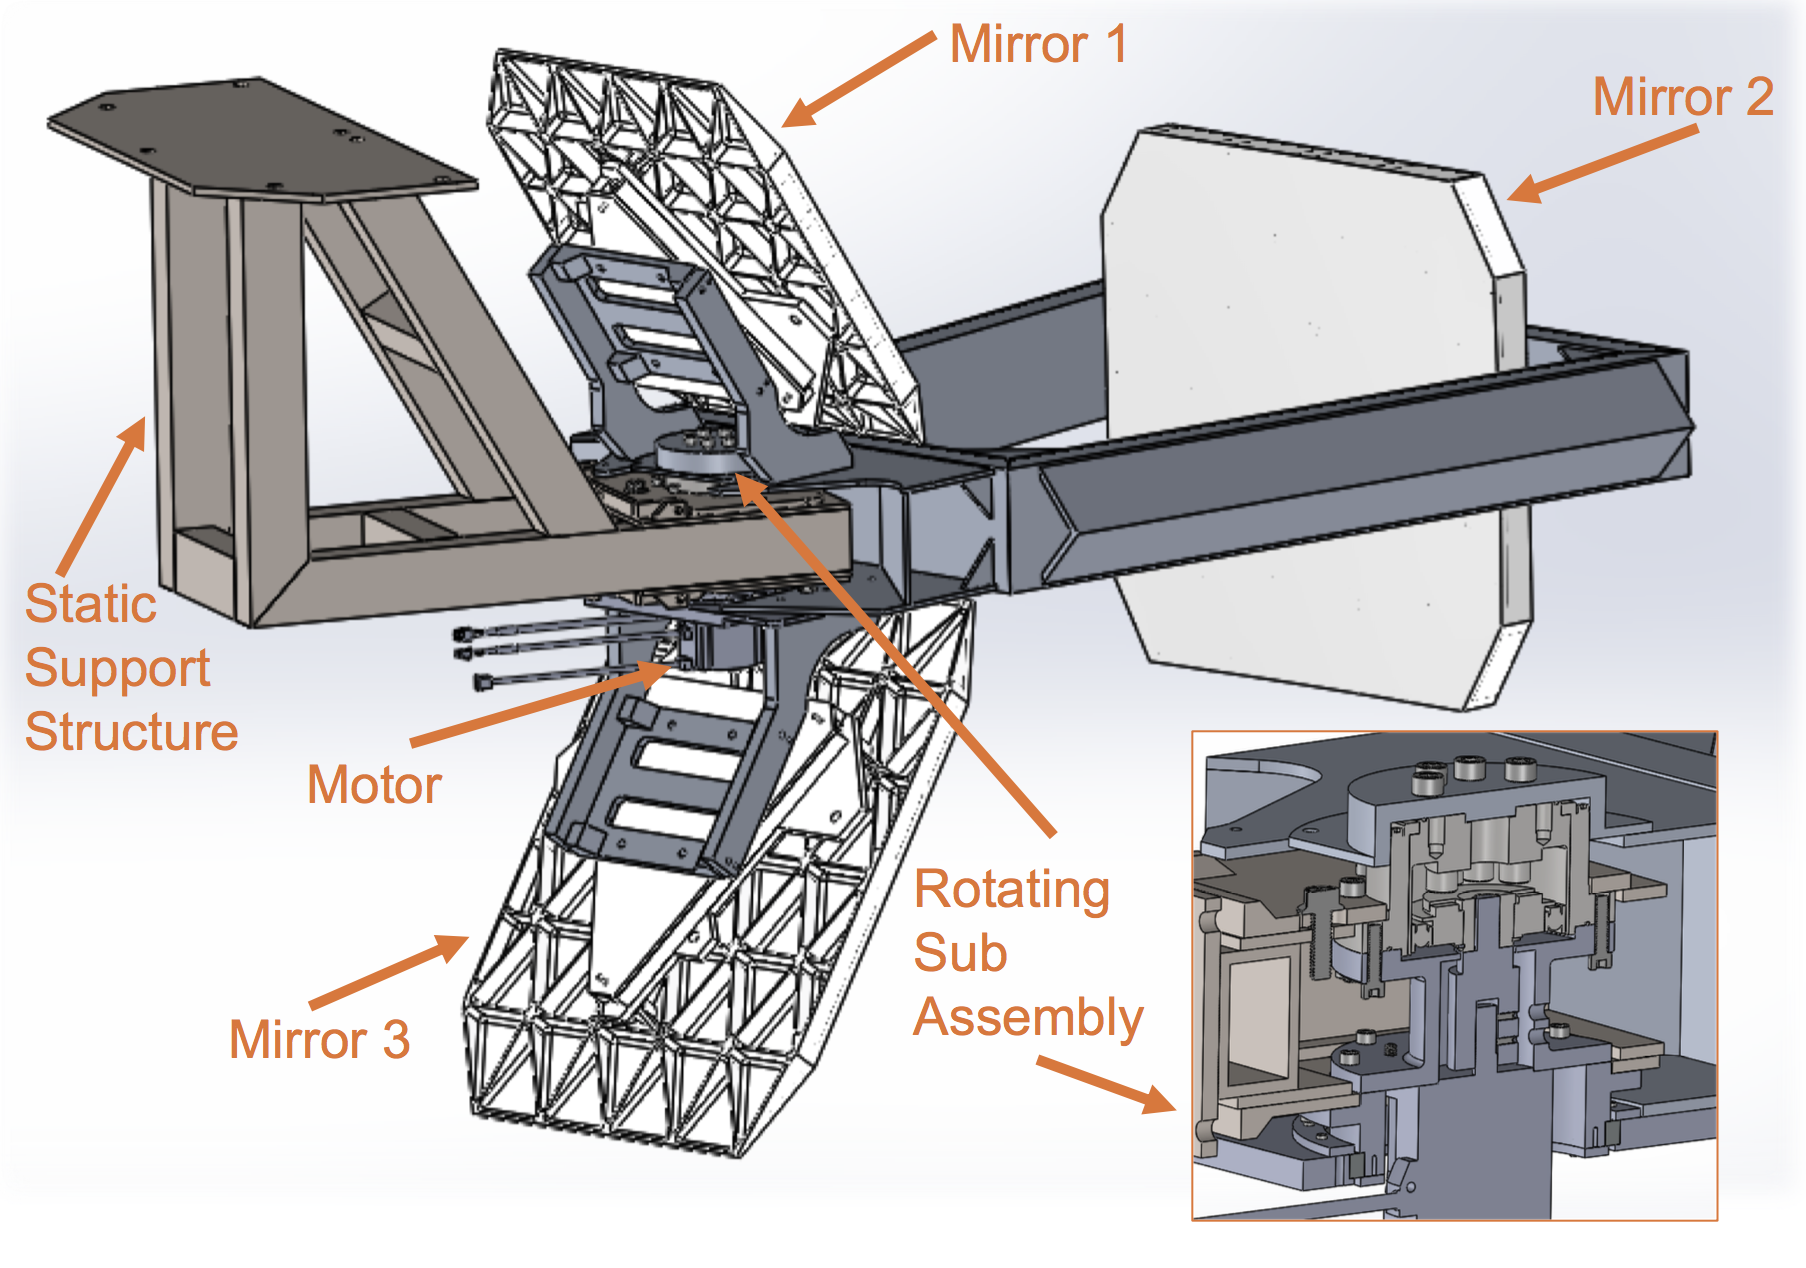
\includegraphics[width=0.45\textwidth]{km2.png} }}%
	\qquad
	\subfloat{{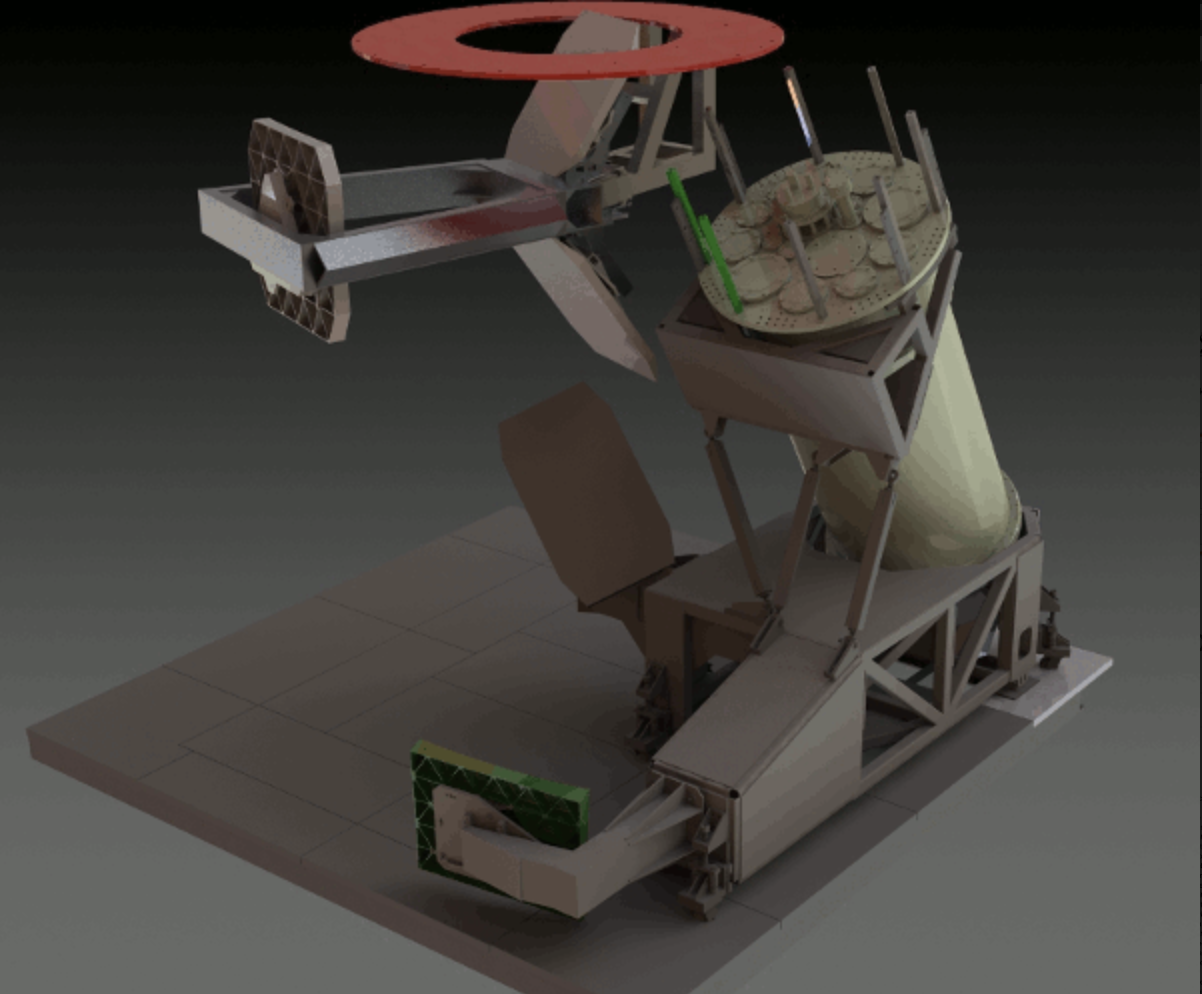
\includegraphics[width=0.45\textwidth]{km3.png} }}%
	\singlespace
	\caption[CAD Model of the K-Mirror Structure.]{Left: The K-Mirror structure consists of three main elements; the support structure made out of 80:20 aluminum, the mirrors, and the motor-gearhead-encoder rotation assembly. Right: The KMS attached inside in the telescope cabin to the flange (red circle) which is the optical input from the secondary mirror. Also shown is the TIME cryostat containing the instrument.}%
	\label{fig:km23}%
\end{figure}

This system is slaved to the motion of the telescope continuously, whether it is moving itself up to scanning position, tracking during an observation, or even in parked mode. Because of this, the telescope sends TCP/IP packets over an ethernet connection containing it's current position and status flags directly to the K-Mirror control computer (Raspberry Pi 3). The motor and gearhead moving the system keep track of their position using an absolute encoder, which states the exact position attained by the system relative to the desired. After receiving the telescope data packets, an internal script is run that calculates the exact amount of rotation that is required to correct the image, based on the current position coordinates. This rotation is actually a well defined term in the field of Astronomy, known as parallactic angle. This angle describes the rotation of the object on the celestial sphere, where zero degrees of rotation is achieved when the object is at the local zenith. As the object travels before and behind zenith, the angle of rotation becomes more positive and more negative respectively. The equation which calculates this angle depends on the latitude of the observer, the hour angle (a function of the local sidereal time), and the declination of the object on the sky. This would mean that the parallactic angle for an object is completely unique for each observing site. Values for the K-Mirror were calculated using position coordinates for Kitt Peak, where it will eventually be deployed. The equation is given below, which was taken from \cite{Meeus1998}.
\begin{equation}
tan(q) = \frac{sin(HA)}{tan(LAT)cos(DEC) - sin(DEC)cos(HA)}
\end{equation}
Here q is the parallactic angle, HA is the hour angle, LAT is the latitude, and DEC is the object declination. While this is the exact version, the actual calculation was performed in python, using the Astropy and Astroplan Packages. These were used because both can calculate the local sidereal time, hour angle, and recalculate object positions entirely from the observers positions and which object position they are starting with, and the starting observation time. Calculation of the local sidereal time (used to calculate the hour angle) was particularly helpful, as this value has complex perturbation errors from nutation in longitude and the true obliquity of the ecliptic that must be included for extremely high precision. The first accounts for the ``wobble" of the earth's axis caused by the moon, with some components having periodic fluctuations on the order of days. The second refers to the difference between the equator and the ecliptic, and how that distance is variable with time. 

The equation above also highlights an important situation which is when the numerator and denominator are zero. This is the case when the object is directly on the zenith of the observer. For this unique position, the equation is undefined, and the object jumps quickly from an angle of $- 90^{\circ}$ to $+ 90^{\circ}$. Movement of that nature for the K-Mirror system (KMS) would be disastrous. The total weight of the system combined with the torque limits of the motor would make a huge jump impossible for the KMS to achieve in a reasonable amount of time, and would probably result in motor failure. Solutions to this problem were three-fold, one set of checks was put in software, another was in hardware, and the last was mapping which observing regions would contain these problem areas. The easiest was hardware, which involved a hard stop limiter that would be tripped if the KMS attempted to move outside of a safe set of ranges. If one of these limit switches was tripped, an error flag would be sent to the command computer, and the system would be stopped. This was meant to be a last resort. In software, the system was designed to prevent over rotation, and rotation too quickly.

The most efficient way of avoiding problems near zenith was to determine at what positions and times objects in the sky at Kitt Peak would pass through the meridian. 
\begin{wrapfigure}{r}{0.5\textwidth}
\vspace{-0.8cm}
  \begin{center}
    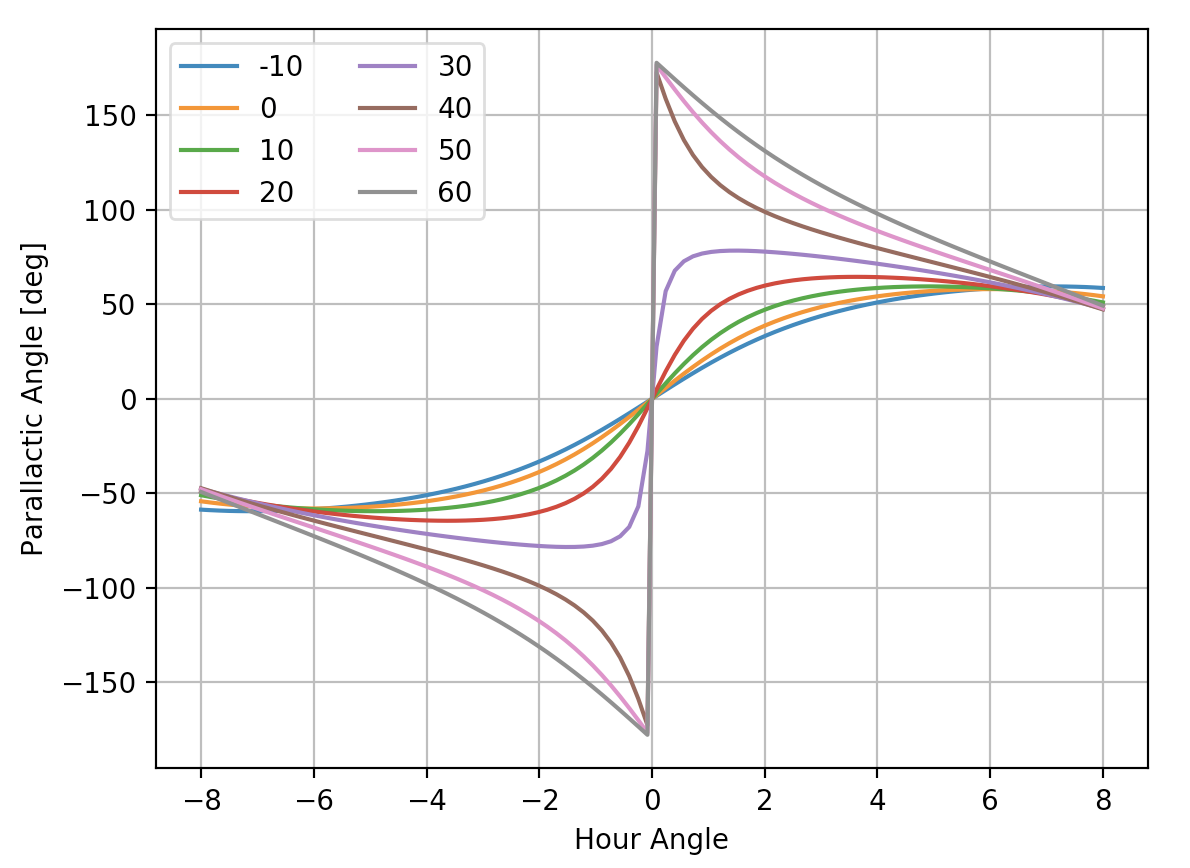
\includegraphics[width=0.48\textwidth]{km6.png}
  \end{center}
  \caption[]{}
  \label{fig:km6}
\end{wrapfigure}
Two difference visualizations were made to assist in determining these problem areas. Figure ~\ref{fig:km6} revealed that for a starting observation of local midnight, the KMS could only observe continuously for roughly 6 hours before it would reach local zenith. The left graph of Figure ~\ref{fig:km45} shows for the same period of time, at what coordinates on the sky those zenith positions are located. The right graph is a comparison for the physical location of the second mirror arm in the cabin at zenith. Any position below 25 degrees in declination appeared to be safe at all times of the night. 

\begin{figure}[ht!]
	\centering
	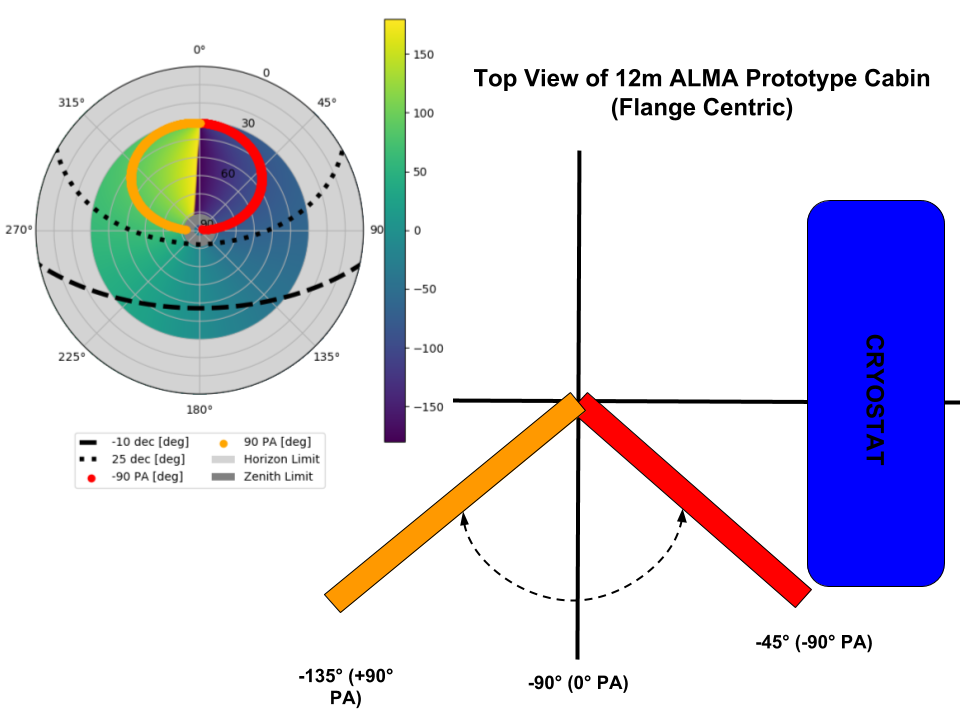
\includegraphics[width=\textwidth]{km45.png}%
	\caption[Parallactic Angle Graphs to Determine Zenith Positions]{Left: Any region on the sky, as viewed from the telescope, that reaches $-90^{\circ}$ or $+90^{\circ}$ PA would require a wrap of the K-Mirror arm back through $0^{\circ}$ PA, which would involve a minimum $45^{\circ}$ rotation. Right: The colors of the arms correspond to the lines of the same color on the plot. }%
	\label{fig:km45}%
\end{figure}

\subsection{Design and Testing}

Two different tests have been run on the software, one which tested exclusively the ability to manipulate the given data and produce corrections in rotation and speed, and the other with a more realistic simulation and use with the motor and encoder. The first test was run with a simulation which mimicked the telescope moving back and forth in a straight line. The top left of Figure ~\ref{fig:km78} shows the absolute position as reported by the simulated telescope, with a change in direction clearly shown halfway through. The error graph shows an average offset of the KMS from the desired position of 14 arcseconds, with a maximum error of 100 arcseconds. The third plot is the reported motor speed, and the last graph is the software attempting to compensate for varying speeds of data packets and updates from the telescope. There are two different types of errors being corrected for here. One is the inability of the KMS to correct for differences in the actual versus desired rotational position, and the other is caused by the variability of the telescope data. In the telescope data transfer is some intrinsic noise caused by the data packets arriving at variable speeds, the updates each having a different values, the imperfect speed of the telescope, and the variable response of the KMS. For example, there are certain circumstances where the telescope may send updates at a rate of 40 packets per second, and have such a slow speed that an update to the position of the KMS is not required at each update, and the update in a position is required at the 29th packet. The transition from stationary to moving is jarring for both the software and mechanical system. 

\begin{figure}[ht!]
	\centering
	\subfloat{{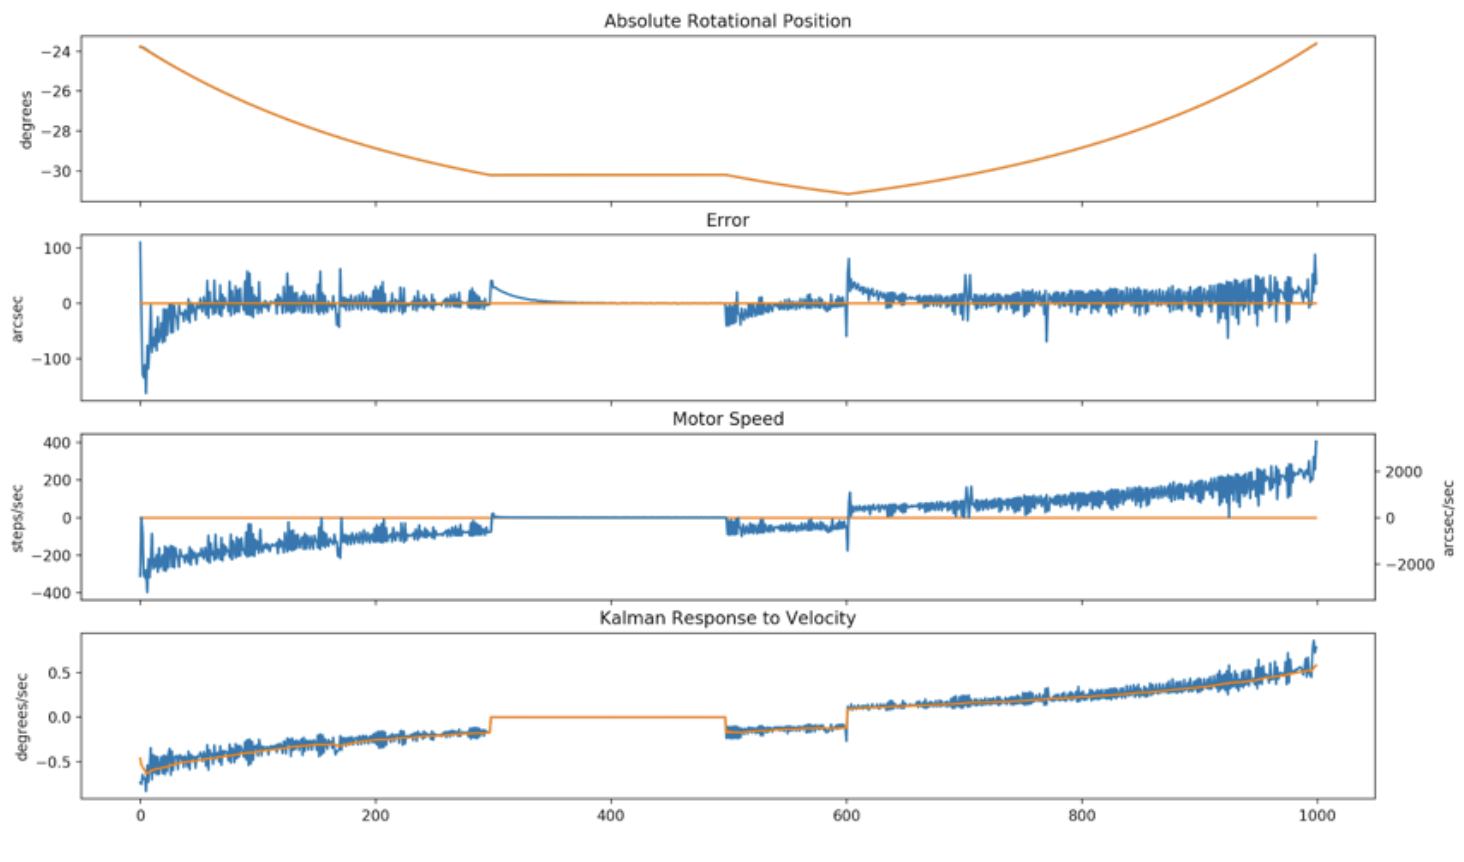
\includegraphics[width=0.45\textwidth]{km7.png} }}%
	\qquad
	\subfloat{{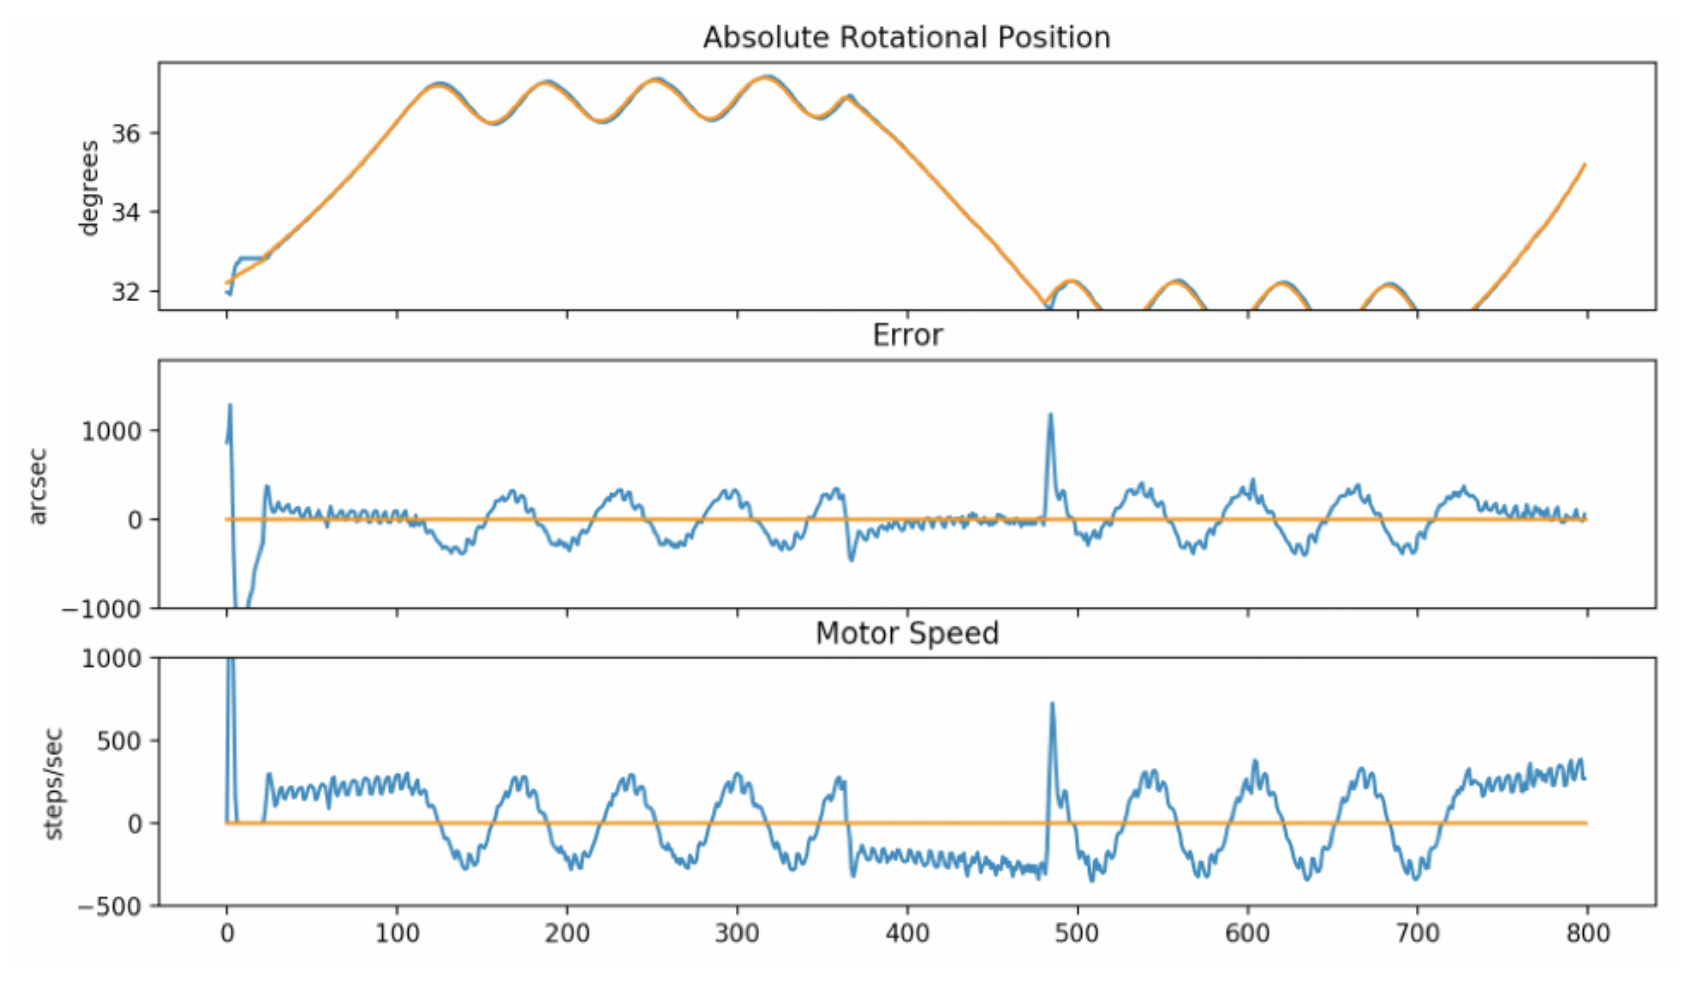
\includegraphics[width=0.45\textwidth]{km8.png} }}%
	\singlespace
	\caption[Telescope Simulation test of KMS Software and Motor]{Both: The orange lines are the information delivered from the telescope, while blue is the response of the KMS. Error graphs refer to the difference in arcseconds between the KMS and calculated position. Left: Simulation showing the KMS software response to telescope input at sidereal rate, 20 packets per second data rate, and a box scan. Right: Simulation showing the KMS motor, encoder and software response from telescope input at 5'' - $1^{\circ}/s$, 20 packets per second data rate}%
	\label{fig:km78}%
\end{figure}

To address this, a Kalman Filter [CITE REFERENCE HERE] was applied to interpret the telescope data based on data rate, relative velocity changes, and the total change in position required. This algorithm creates an unbiased estimate of the natural ``noise'' of the telescope-K-Mirror system, and then continually correct the data for this average error, and updates this average error over a period of time. This allowed the motor to more smoothly start and stop, and improved the ability of the software to correct for changes in observational modes. The right graph of Figure ~\ref{fig:km78} shows this improvement on the actual motor, gearhead and encoder with a more sophisticated telescope simulator. In the first simulation, the telescope speed was set to the sidereal rate, with a box-like pattern of motion set of coordinates provided to the KMS. The second simulation included a ``slewing'' phase, where the telescope was moving at 1 degree per second up to a starting position, and then a ``tracking'' phase at 5 arcseconds per second, where the telescope was moving back and forth across the given coordinates. This scenario produced the sort of line scan that TIME will be using to move back and forth across a cluster source as it moves through the sky from the earths rotation, and at roughly the correct observing speeds. This test proved that the software and motor was capable of keeping up with the telescope even at its fastest speed while also reducing error to within tolerances.  Additional testing includes adding the mirror mass models and test the software and motor under a load bearing case, and attempt to simulate the data transfer from telescope to KMS over an isolated network server. A script designed to simulate telescope socket data transfer has already been written by the University of Arizona but has not yet been tested. 

\subsection{Software Integration}

The KMS software was designed to integrate with the GUI in order to facilitate real-time monitoring of its status. It receives input directly from the telescope, but only sends output to the control computer. This includes several flags for emergencies, like ``emergency stop'', ``standby'', and ``rotating''. There is no way for the control computer to directly communicate with the KMS, and instead will be done by way of the telescope. This reduces the complexity of code necessary for controlling the KMS, reduces the load on the Raspberry Pi 3, and creates less opportunity for software malfunction. In a situation where there is a problem with the KMS, MCE, detectors, or any other connected component to the control computer, an emergency stop button can be pressed on the GUI, which will send a signal to simultaneously stop all other processes (i.e. telescope motion, data acquisition, etc.) Additionally, the current parallactic angle will be output on the screen next to the angle achieved by the KMS, as well as the current speed. Currently, the telescope data has not been added to the GUI, but since the data flow exists in that direction, information could be sent that includes current pointing coordinates, average speed, current time (UTC), and possibly also a status flag stating what mode it is in. 


%%%%%%%%%%%%%%%%%%%%%%%%%%%%%%%%%%%%%%%%%%%%%%%%%%%%%%%%%%%%%%%%%%%%%%%%%%%%%%%%%%%%%%
%%%%%%%%%%%%%%%%%%%%%%%%%%%%%%%%%%%%%%%%%%%%%%%%%%%%%%%%%%%%%%%%%%%%%%%%%%%%%%%%%%%%%%

\section{In Conclusion}

The TIME instrument will be integral to creating the first large sky survey of the kSZ effect, and improving upon measurements of CII and CO line intensities in galaxies and galaxy clusters. To accomplish this, it will be using a driven scan intensity mapping observing strategy, which has the advantages of quick integrations times, and a low spatial resolution, without the need to resolve individual galaxies. It will also be able to successfully remove atmospheric contamination from the data, and any other systematic noise, by taking multiple measurements of the same patch of sky across its 16 detectors. These improvements have the potential for many scientific insights, briefly summarized again below.

The kSZE will be mapped across multiple redshifts to a high significance, creating the first peculiar velocity maps of large scale structure. This map will be able to trace the gravitational potentials through cosmic time, without any dependence on the redshift being observed. From this we can generate theories about the role of dark matter production in the early universe and how it influenced the development of gravitational perturbations to the space-time metric. Dark matter is currently theorized to contribute 25\% of the matter energy density of the universe, which has been estimated from the anisotropies in the CMB and other methods. With this additional method of visualizing dark-baryonic matter interactions, these values can be corroborated through an independent technique. 

One additional use for observing kSZE is in determining the gas physics at work in the ICM. Since we are essentially measuring the motion, temperature, and possibly feedback and cooling outflows of the gas, a model for the hydrodynamical evolution of cluster gas with redshift can also be created. This is especially useful as a comparator to other cluster measurement techniques that rely heavily on the assumed gas clumping and density. More often these values are taken from local sources that may create some redshift correlated error when used outside the local cluster. This insight into gas dynamics is a shared trait with CII and CO measurements. While kSZE focuses mostly on the ICM, CII and CO can also reach the ISM and IGM (for isolated galaxies). In this case, the usefulness is in studying the transition of galaxies through the Epoch of Reionization and the Epoch of Peak Star Formation. CII can probe the ionized medium, while CO traces the neutral hydrogen reservoirs. The combination can reveal the ionization bubble size and development around primordial galaxies, the physics of the first ionizing sources, show the changing neutral gas reservoirs in galaxies, and allow modeling of changing stellar populations at different epochs. 

It is clear from the discussion above that TIME will have numerous contributions to the field of Cosmology, which is somewhat astounding considering it is all possible from a single experiment. Provided everything goes well, it should be making strides as early as the winter of 2018, with results from data analysis possibly a year after. The writer will be holding their breath in anticipation. 

%%%%%%%%%%%%%%%%%%%%%%%%%%%%%%%%%%%%%%%%%%%%%%%%%%%%%%%%%%%%%%%%%%%%%%%%%%%%%%%%%%
% REFERENCES
\newpage
\renewcommand\bibsection{\section{\refname}}
\bibliographystyle{unsrtnat}
\bibliography{references}

\newpage
\appendix


\end{document}
